\documentclass[aspectratio=1610]{beamer}
\usepackage{ctex, hyperref, ulem}
\usepackage{fbox, fancyvrb}
\usepackage[T1]{fontenc}

% other packages
\usepackage{latexsym,amsmath,xcolor,multicol,booktabs,calligra}
\usepackage{graphicx,pstricks,listings,stackengine}

\author{张智豪\inst{1} \and miyou379\inst{2}}
\title{A Tour of ?}
\subtitle{Network,Operating System,Programming Languages}
\institute
{
    \inst{1}
    School of Accountancy\\
    Southwestern University of Finance and Economics
    \and
    \inst{2}
    Code All Accepted Group
}
\date{October,2024}
\usepackage{Tsinghua}

\hypersetup{
    colorlinks=true,
    linkcolor=blue,
    urlcolor=blue,
    citecolor=green,
}

% defs
\def\cmd#1{\texttt{\color{red}\footnotesize $\backslash$#1}}
\def\env#1{\texttt{\color{blue}\footnotesize #1}}
\definecolor{deepblue}{rgb}{0,0,0.5}
\definecolor{deepred}{rgb}{0.6,0,0}
\definecolor{deepgreen}{rgb}{0,0.5,0}
\definecolor{halfgray}{gray}{0.55}

\lstset{
    basicstyle=\ttfamily\small,
    keywordstyle=\bfseries\color{deepblue},
    emphstyle=\ttfamily\color{deepred},    % Custom highlighting style
    stringstyle=\color{deepgreen},
    numbers=left,
    numberstyle=\small\color{halfgray},
    rulesepcolor=\color{red!20!green!20!blue!20},
    frame=shadowbox,
}


\begin{document}

\begin{frame}
    \titlepage
\end{frame}

\begin{frame}
    \tableofcontents[sectionstyle=show,subsectionstyle=show/shaded/hide,subsubsectionstyle=show/shaded/hide]
\end{frame}


\section{何为CS?}

\begin{frame}[c]{程序员的三大浪漫\ 轮子哥(\href{https://www.zhihu.com/people/excited-vczh}{@vczh})}
    \begin{itemize}[]
        \item 操作系统
        \item 图形可视化
        \item 编译原理
    \end{itemize}
\end{frame}

\begin{frame}[t]{计算机科学的分类}
    \fparbox[Br,boxrule=5pt,boxsep=10pt]{\textrm{\textit{There are only two hard things in Computer Science: cache invalidation and naming things.}}\hfill-- \href{https://martinfowler.com/bliki/TwoHardThings.html}{Phil Karlton}}
    
    \begin{block}{Disciplines}
        理论计算机科学、计算机系统、计算机应用、软件工程\footnote{\href{https://en.wikipedia.org/wiki/Computer_science}{Computer science} - Wikipedia}
    \end{block}

    \begin{center}
        \begin{itemize}
            \item<1-> 可计算理论、信息论与编码、数据结构与算法、形式语义...
            \item<2-> 并行计算、系统架构、操作系统、RTOS、网络工程...
            \item<3-> 可视化、图像处理、AI、数据处理、科学计算...
            \item<4-> 设计模式、设计思维...
        \end{itemize}
    \end{center}
    
    \only<1>{更多的数学,形式化定义,更多的抽象思维}
    \only<2>{更多的硬件机制,更多的 \href{https://pubs.opengroup.org/onlinepubs/9799919799/index.html}{Conventions} 和 Manuals}
    \only<3>{大部分均为学科交叉,已经形成了自己较为独立的知识架构}
    \only<4>{强调自动化的工具使用,思想的落实实现}

    
\end{frame}

\section{网络}

\begin{frame}[t]{IP地址与DNS}
    \fparbox[Br,boxrule=5pt,boxsep=10pt]{\textrm{很久很久以前,每个人都没有名字...称呼只能用“你我他”}}

    \begin{center}
        \begin{itemize}
            \item 名字的重要性
            \item 如何确保每个人的名字是唯一的?
            \item 这个问题该丢给ISP来处理
        \end{itemize}
    \end{center}

    \alert{IP地址}是每台计算机在网络上的身份证号,有了它你能够精准无误的找到任何一台连接到因特网的电脑 \\[1em]
    
    那么代价是?
    \begin{center}
        \begin{itemize}
            \item 冗长的IP地址需要记忆
            \item IP地址也是一种\alert{网络资源}!!
        \end{itemize}
    \end{center}
\end{frame}

\begin{frame}[t]{IP地址与DNS (cont'd)}
    \alert{DNS}(Domain name server)解决了网址与动态域名的映射关系 \\[1em]
    网址是基于HTTP协议的 \href{https://en.wikipedia.org/wiki/URL}{URL}
    
    \begin{figure}[htpb]
        \centering
        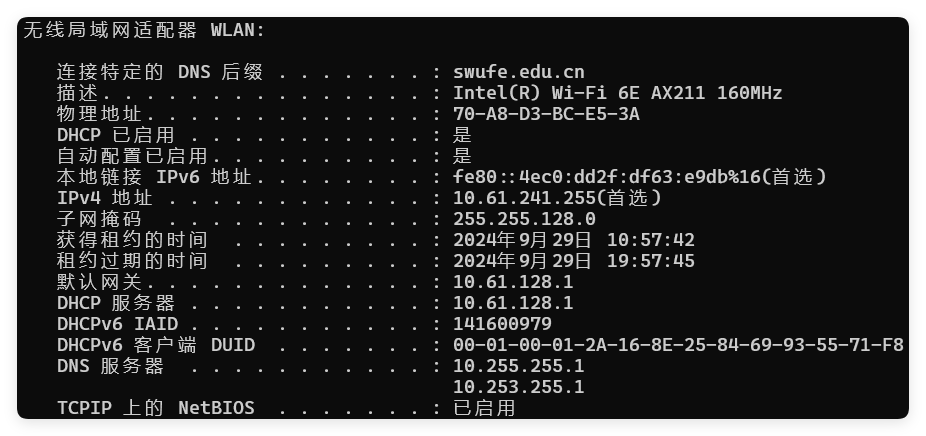
\includegraphics[height=0.6\textheight]{pic/DNS.png}
        \caption{使用\texttt{ipconfig /all}查看DNS服务器}
    \end{figure}
\end{frame}

\begin{frame}[t]{IPv4与子网掩码}
    IPv6号称可以给世界上每一粒沙子一个编号
    \begin{center}
        \begin{itemize}
            \item 然而IP地址变得很长,有128位
            \item 截止到目前纯IPv6网站仍然很少
            \item 西财校园网疑似并不支持(?)
        \end{itemize}
    \end{center}

    考虑到大部分人其实并不需要拥有一个独特的IP地址 \\
    我们可以把许多台电脑组成一个子网 \\
    用一个子网掩码来区分子网当中的不同主机\footnote{\href{https://www.cnblogs.com/tiandi/p/16320212.html}{IP地址、子网掩码、网关、DNS简介} - 博客园} \\[1em]

    习题:\href{https://onlinejudge.org/index.php?option=com_onlinejudge&Itemid=8&page=show_problem&problem=4465}{UVA-1590 IP Network}(注意本题中子网掩码定义略有区别)
\end{frame}

\begin{frame}{Proxy:疑似是敏感的话题}
    网络编程(又称套接字编程)中我们需要把不同的应用程序对应到不同的\href{https://gnu-linux.readthedocs.io/zh/latest/Chapter03/00_port.html}{\alert{端口}}(Port),为系统提供服务\footnote{\href{https://www.iana.org/assignments/service-names-port-numbers/service-names-port-numbers.xhtml}{Service Name and Transport Protocol Port Number Registry} - IANA}\\[0.5em]
    网络回环地址:\href{http://127.0.0.1/}{127.0.0.1}
    \begin{center}
        \begin{itemize}
            \item 真的是它吗?不妨在Docker里面验证一下\footnote{\href{https://kaiyuanshe.feishu.cn/wiki/AUANwul81iwbVSkrzqRcJzVlnAv}{Docker中的localhost、127.0.0.1...} - 开源社}
        \end{itemize}
    \end{center}

    \begin{figure}[htpb]
        \centering
        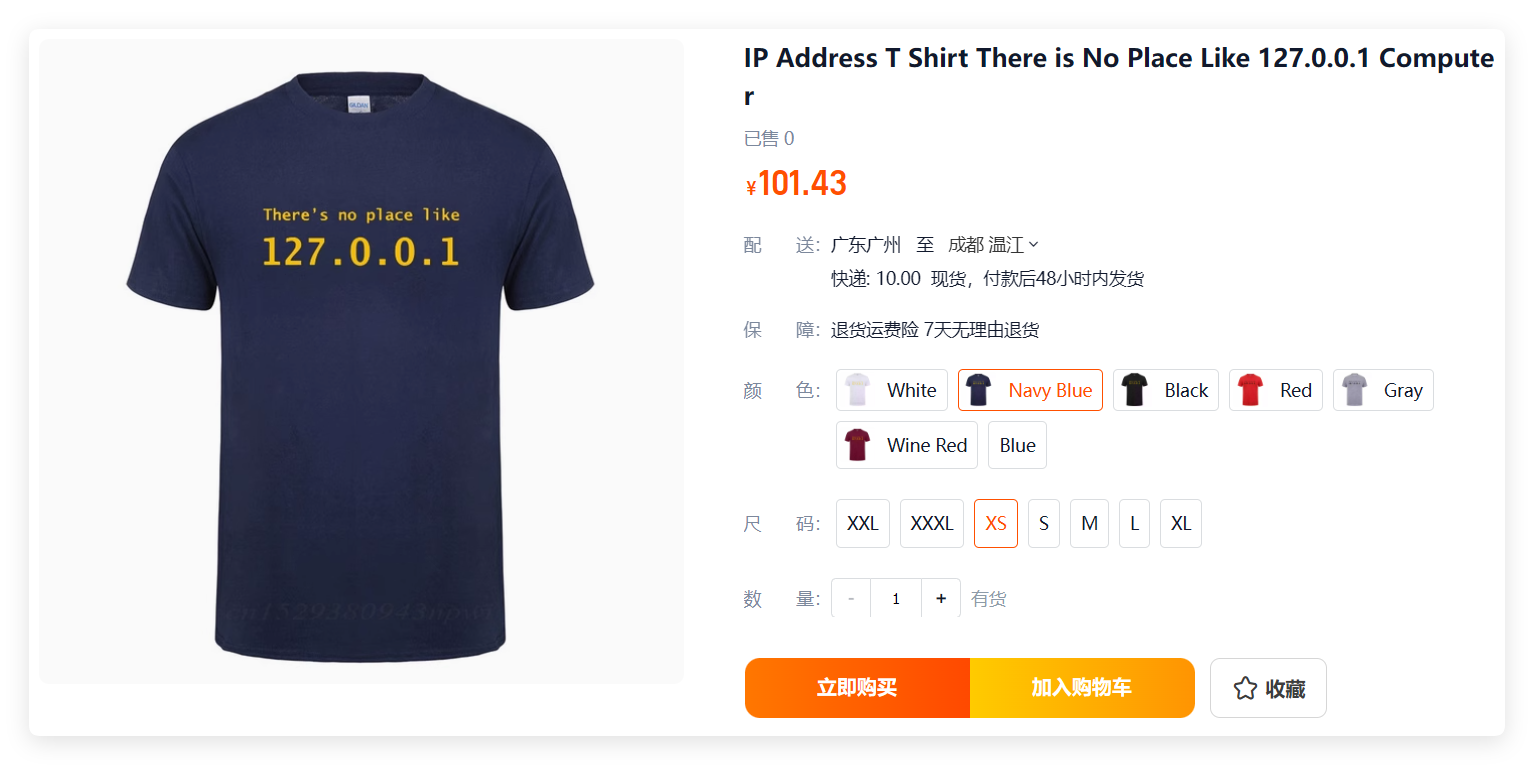
\includegraphics[height=0.5\textheight]{pic/Tshirt.png}
    \end{figure}
\end{frame}

\begin{frame}{Proxy: 疑似是敏感的话题 (cont'd)}
    \begin{minipage}{0.6\textwidth}
        Proxy软件
        \begin{center}
            \begin{itemize}
                \item 小学时候的Shadowsocks
                \item 初中常用的V2ray
                \item 高中开始用的Clash...
            \end{itemize}
        \end{center}
    
        Clash for Windows,ClashX,Clash for Android, \\
        Clash,Clash verge,Clash verge rev傻傻分不清?\\

        系统代理与图形界面和操作系统设计有关 \\
    
        \href{https://en.wikipedia.org/wiki/Virtual_private_network}{VPN} 最早还真不是拿来干这玩意的\footnotemark
    \end{minipage}
    \begin{minipage}{0.34\textwidth}
        \centering
        
\includegraphics[width=\textwidth]{pic/Google.png}
    \end{minipage}

    \footnotetext{{\href{https://webvpn.swufe.edu.cn}{西南财经大学WebVPN}}}
\end{frame}

\section{操作系统}

\subsection{历史背景}

\begin{frame}{What?}
    啥叫 \href{https://en.wikipedia.org/wiki/Operating_system}{Operating system}
    \begin{minipage}{\textwidth}
        \centering
        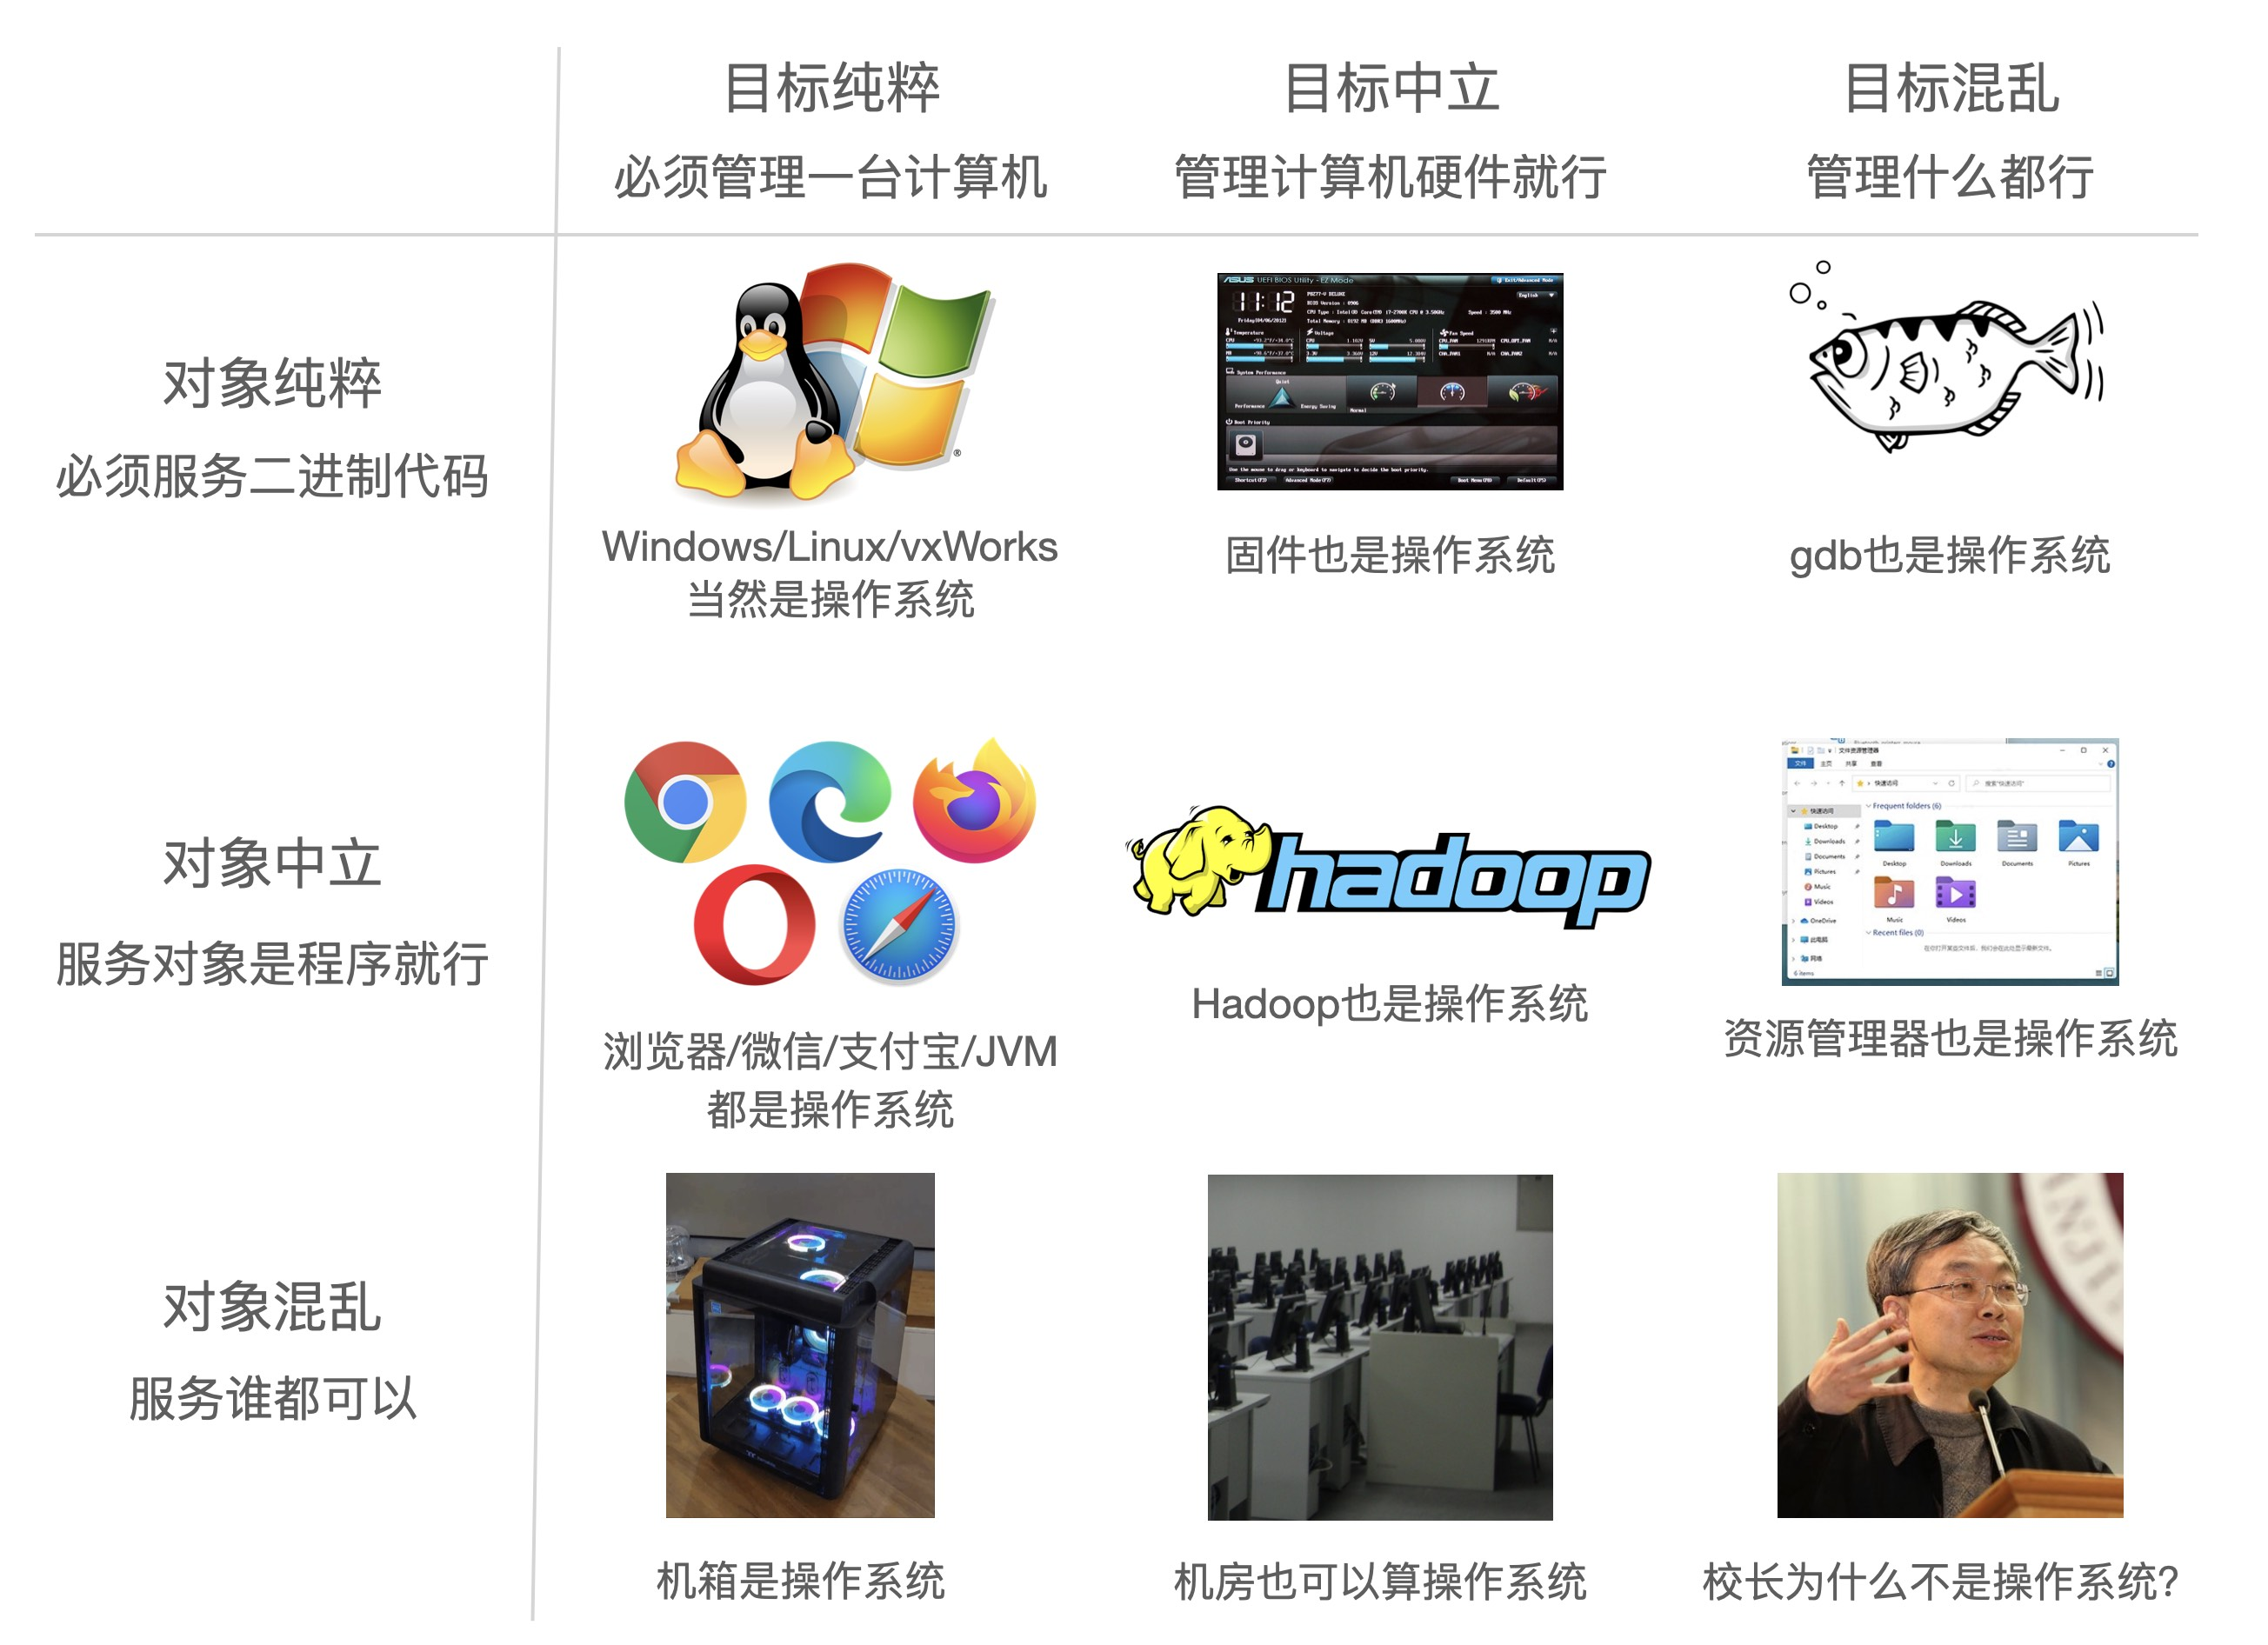
\includegraphics[height=0.5\textwidth]{pic/os-classify.jpg}
    \end{minipage}
\end{frame}

\begin{frame}{1940s: 第一台通用电子计算机ENIAC\footnote{\href{https://www.cs.drexel.edu/~bls96/eniac/}{ENIAC emulator} 和在 \href{https://jyywiki.cn/pages/OS/2022/demos/sieve.e}{ENIAC上跑素数筛}}}
    \begin{itemize}
        \item 为弹道计算而生
        \item 使用旋钮和布线接板进行编程
        \item 输入输出采用IBM的打孔卡片(Punch cards)
        \item 计算已经很吃力,没有操作系统的概念
    \end{itemize}
    \begin{minipage}{\textwidth}
        \centering
        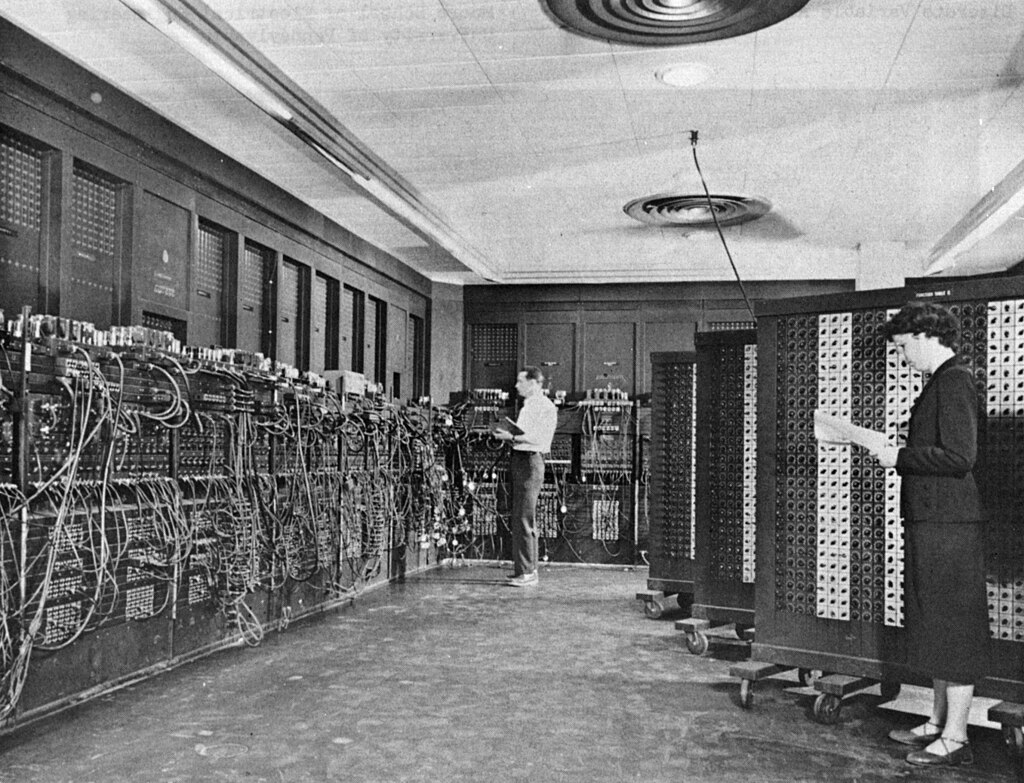
\includegraphics[height=0.32\textwidth]{pic/ENIAC.jpg}
    \end{minipage}
\end{frame}

\begin{frame}{1950s: Fortran出现}
    \begin{itemize}
        \item 不再直接访问硬件
        \item 现在写程序也用打孔卡片,不过是公式化的标准卡片
        \item 额,还是没有操作系统,电脑少用户多,产生了“换卡”的需求
    \end{itemize}
    \begin{minipage}{\textwidth}
        \centering
        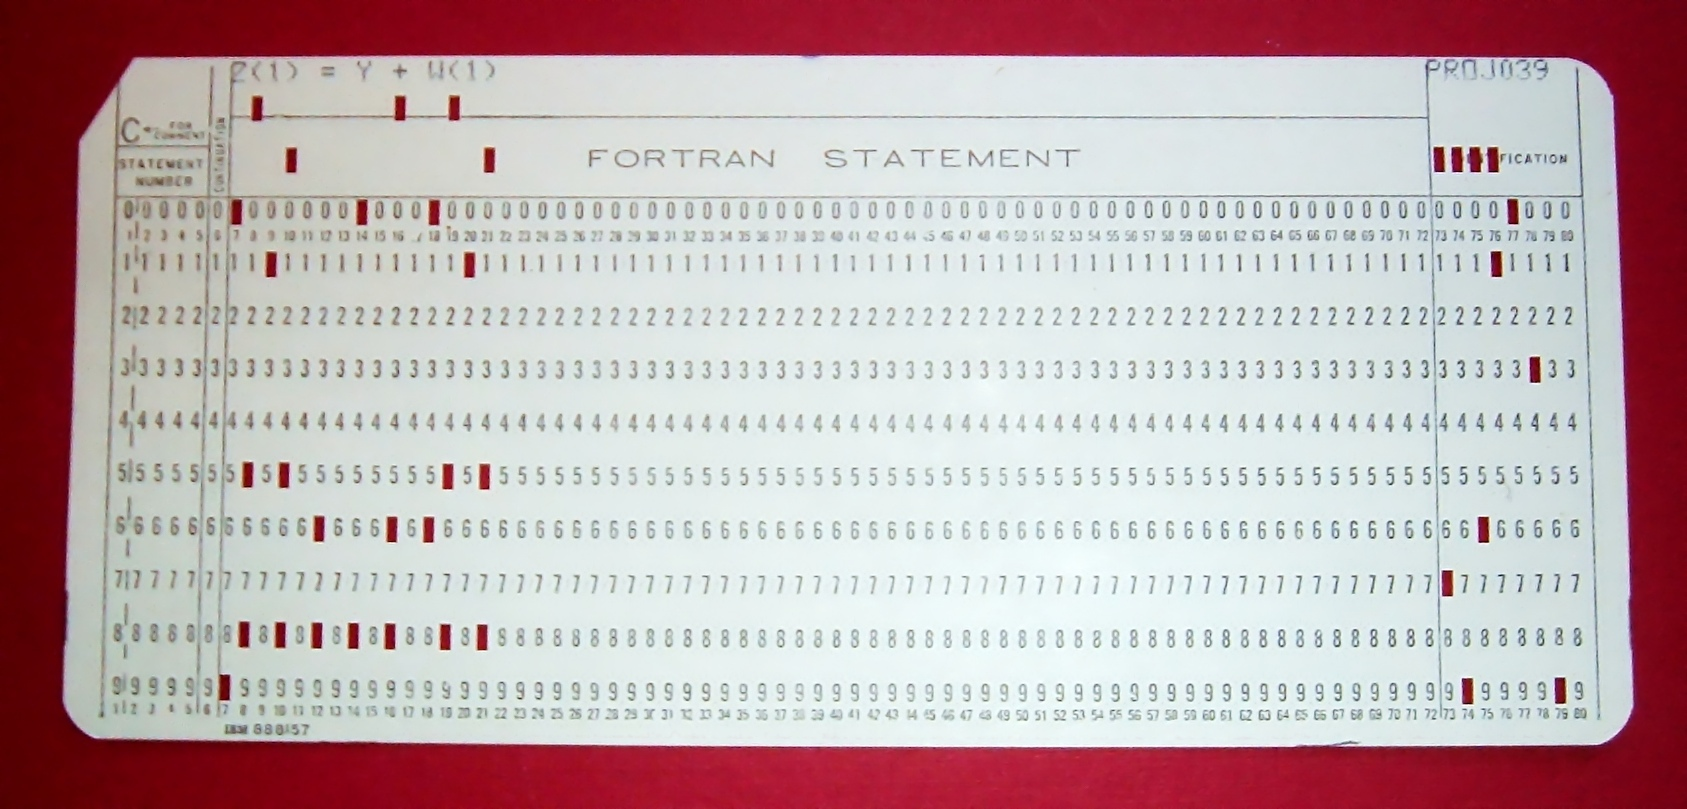
\includegraphics[height=0.35\textwidth]{pic/FortranCardPROJ039.agr.jpg}
    \end{minipage}
\end{frame}

\begin{frame}{1960s: OS/360、Multics}
    为大型机(Mainframe)准备的操作系统
    \begin{itemize}
        \item 集成电路、总线出现,计算机变得空前的tiny,内存变得空前的大
        \item 产生了分时概念,用户只需要在不同的程序之间切换而不用换卡
        \item OS/360是IBM System/360的御用操作系统
        \item \alert{Multics}(MIT)作为最成功的分时模型对现代操作系统拥有决定性影响
        \item Multics(1965)标志着现代操作系统正式诞生
    \end{itemize}
\end{frame}

\begin{frame}{1970s: UNIX(\href{https://en.wikipedia.org/wiki/Ken_Thompson}{\alert{肯·汤姆森和丹尼斯·尼奇}}) Family}
    \begin{itemize}
        \item C语言、PASCAL语言等高级语言出现
        \item \alert{UNIX}(Bell Labs, 1973)\footnote{\href{https://dl.acm.org/doi/pdf/10.1145/361011.361061}{The UNIX Time-Sharing System}} 家族开始引领时代潮流
    \end{itemize}
    \begin{minipage}{\textwidth}
        \centering
        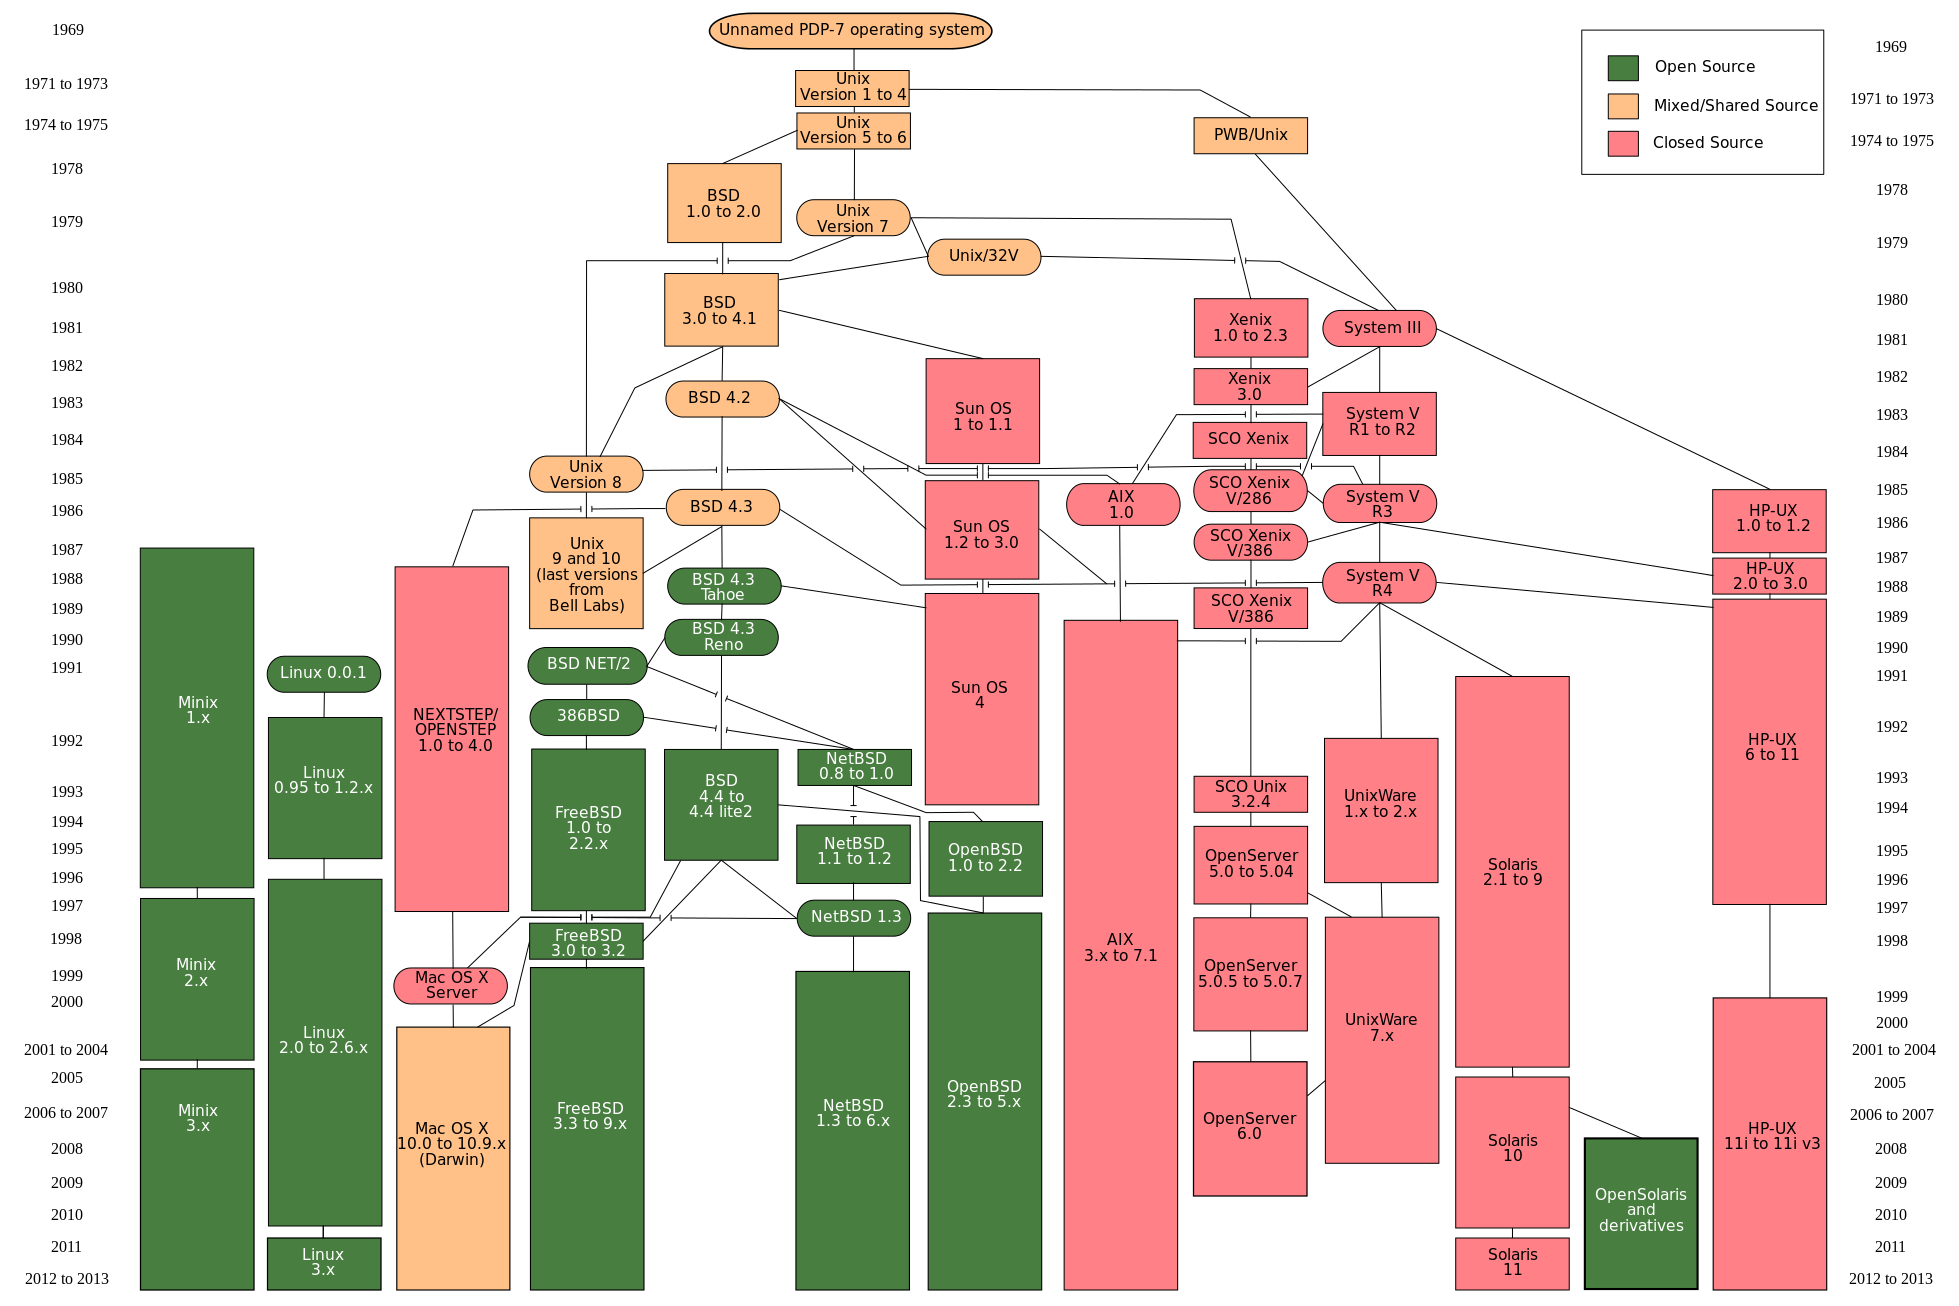
\includegraphics[height=0.43\textwidth]{pic/unix_branch.png}
    \end{minipage}
\end{frame}

\begin{frame}{1980s+: MS-DOS、Linux}
    \begin{itemize}
        \item MS-DOS(1981)\footnote{我知道你们都没学8086汇编,来 \href{https://www.dosbox.com/}{DOSBOX} 玩玩吧!} 作为IBM兼容机的操作系统风靡一时\,推荐动漫\,16bit的感动
        \item Linus Torvalds在大学期间仿照Minix\footnote{传说中的Minix book: \href{https://dl.acm.org/doi/book/10.5555/1076555}{Operating Systems: Design and Implementation}} 写出了Linux内核\enspace 然后和祖师爷对喷\footnote{\href{https://groups.google.com/g/comp.os.minix/c/wlhw16QWltI}{1992年},\enspace\href{https://www.realworldtech.com/forum/?threadid=65915&curpostid=65936}{2006年}在论坛喷人}
    \end{itemize}
    \begin{minipage}{\textwidth}
        \centering
        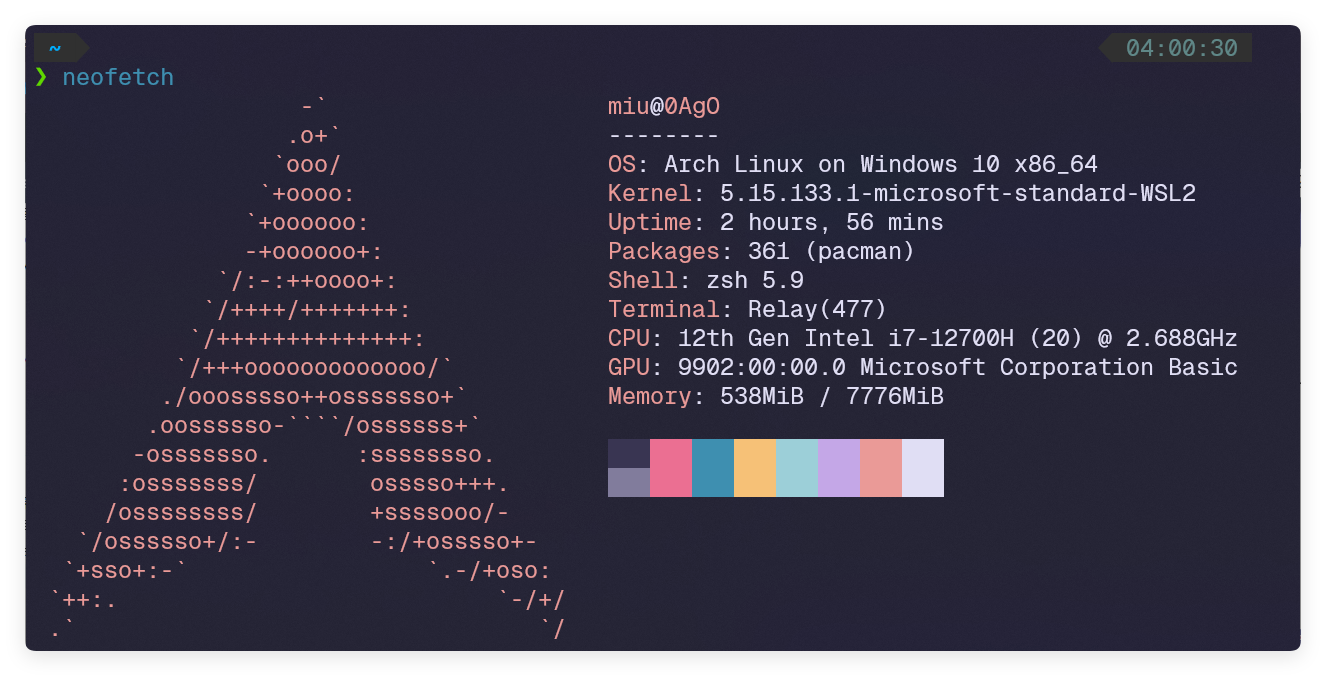
\includegraphics[height=0.35\textwidth]{pic/ArchLinux.png}
    \end{minipage}
\end{frame}

\begin{frame}[t]{2000s+: Windows NT、各种Linux发行版}
    \begin{minipage}{0.6\linewidth}
        \centering
        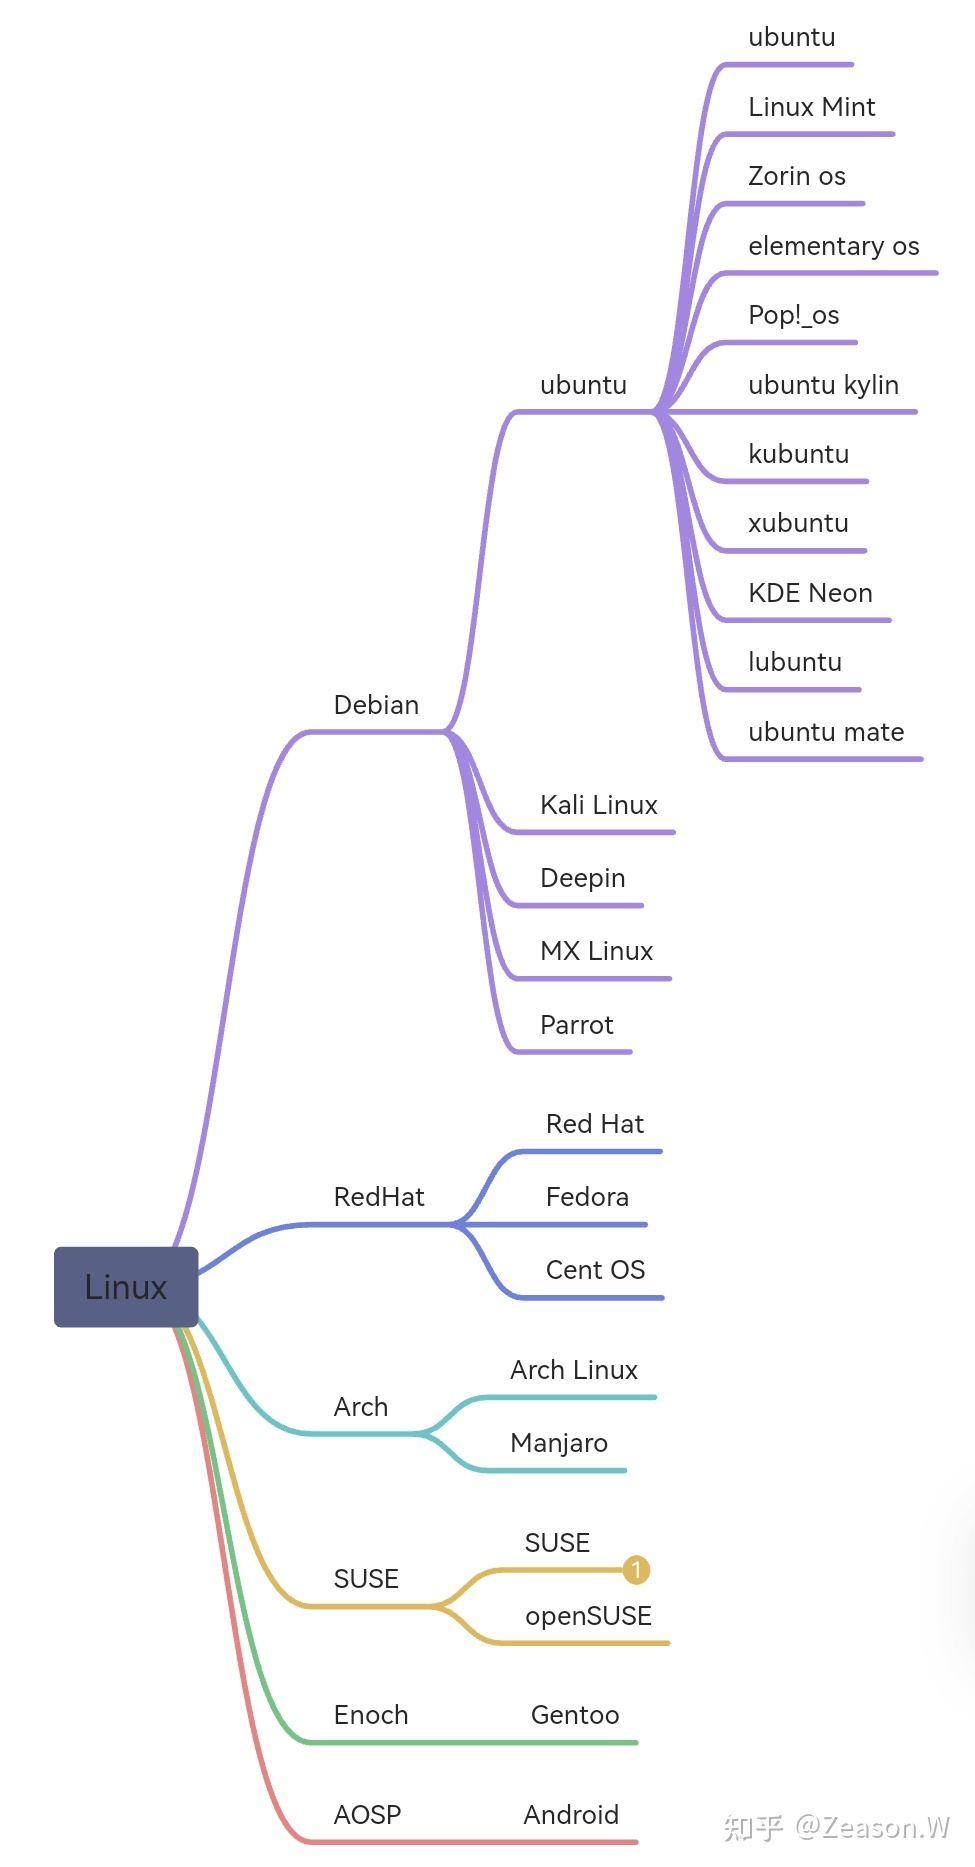
\includegraphics[width=0.45\linewidth]{pic/linux_branch.jpg}
    \end{minipage}
    \begin{minipage}{0.3\linewidth}
        \begin{center}
            \href{https://zhuanlan.zhihu.com/p/549547091}{MS-DOS与Windows与WindowsNT}
        \end{center}
    \end{minipage}
\end{frame}

\subsection{开源项目}

\begin{frame}[t]{Rising for operating system: The GNU project}
    \fparbox[Br,boxrule=5pt,boxsep=10pt]{\textrm{The GNU Operating System and the Free Software Movement}}\newline
    
    递归缩写:GNU's not UNIX!
    \begin{center}
        \begin{itemize}
            \item 由 \href{https://www.stallman.org/}{Richard Matthew Stallman}(\sout{抠脚大叔})发起
            \item GNU计划下的软件都遵循 \alert{GPL开源协议}\footnote{\href{https://opensource.org/license/gpl-2-0}{GNU General Public License version 2}}
            \item 更多的思想碰撞\footnote{\href{https://www.bilibili.com/video/BV1oo4y1x7Nw}{The Tragedy of systemd} - Benno Rice}
        \end{itemize}
    \end{center}

    你现在用的Linux不叫Linux,叫做 \alert{GNU/Linux}!
    \begin{center}
        \begin{itemize}
            \item GNU/Linux下的所有软件和工具全部来自GNU计划,并保证是完全“自由”的
            \item 没有这些工具,你能玩的只有一个Linux kernel;GNU也有自己的OS(内核)\footnote{\href{https://www.gnu.org/software/hurd/hurd.html}{GNU Hurd}}
        \end{itemize}
    \end{center}
\end{frame}

\begin{frame}{开源协议声明了什么?}
    允许了什么?
    \begin{itemize}
        \item 新的发行版(众多的GNU/Linux发行版)
        \item \alert{商业化使用}(Qt与亲儿子KDE Desktop\footnote{\href{https://userbase.kde.org/History_of_KDE/zh-cn}{KDE的历史} - KDE UserBase Wiki})
        \item 对原有软件的修改和添加(RHEL不再公开源代码\footnote{\href{https://www.theregister.com/2023/06/23/red_hat_centos_move/}{Red Hat strikes a crushing blow against RHEL downstreams} - The Register, 2023})
        \item 甚至是专利权?或者用你的名义打广告?(\href{https://opensource.org/license/bsd-3-clause}{BSD 3-Clause License})
    \end{itemize}
\end{frame}

\begin{frame}[t]{让人头大的图形界面...}
    \fparbox[Br,boxrule=5pt,boxsep=10pt]{\textrm{\alert{Shell} \footnote{\href{https://superuser.com/questions/144666/what-is-the-difference-between-shell-console-and-terminal}{What is the difference between shell, console and terminal?} - StackExchange} 是操作系统心灵的窗口}\hfill-- miyou379}\newline

    \begin{minipage}{0.6\linewidth}
        UNIX shell
        \begin{center}
            \begin{itemize}
                \item 最早的:汤姆森shell(sh)
                \item 以前最盛行的:Bourne shell(sh)
                \item GNU的:Bourne-Again shell(bash)
                \item 最用户友好的:Fish shell(fish)
                \item 拓展性极高的:Z-Shell(zsh)
            \end{itemize}
        \end{center}
        \href{https://en.wikipedia.org/wiki/Cmd.exe}{\alert{CMD.exe}} 和 \href{https://en.wikipedia.org/wiki/PowerShell}{\alert{PowerShell}}
    \end{minipage}
    \begin{minipage}{0.35\linewidth}
        \centering
        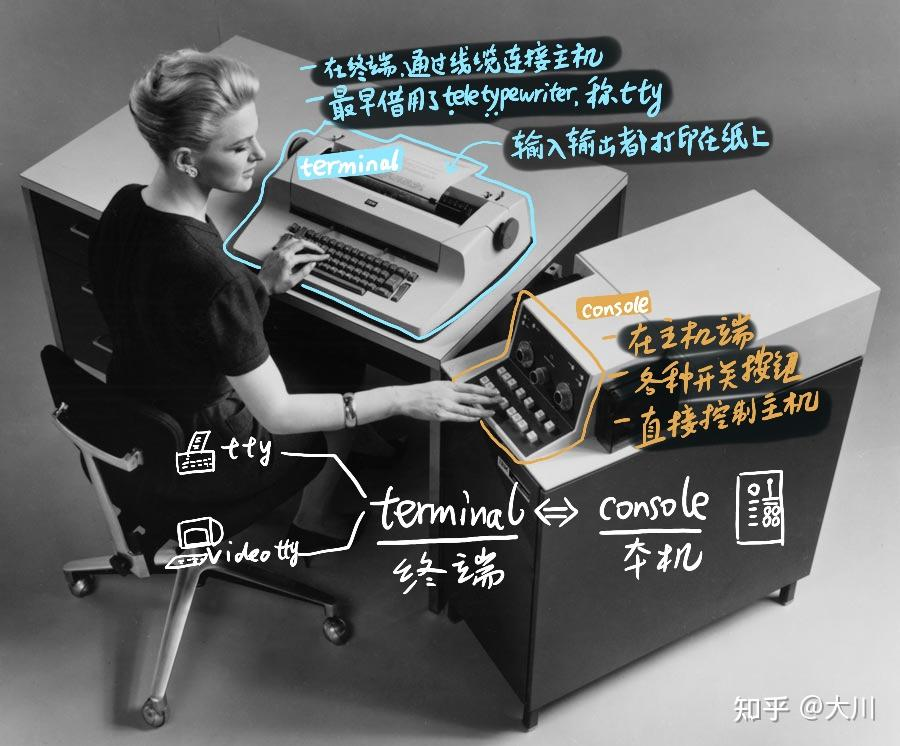
\includegraphics[width=\linewidth]{pic/operate.jpg}
    \end{minipage}

    \footnotetext{\href{https://linux.cn/article-14093-1.html}{Linux 黑话解释:TTY 是什么?} - Linux中国}
    \footnotetext{\href{https://www.zhihu.com/question/21711307/answer/2231006377}{终端、Shell、tty 和控制台(console)有什么区别?} - 大川的回答 - 知乎}
    \footnotetext{\href{https://b23.tv/FeXYJbj}{[Thermal TTY]用热敏打印机和Arduino制作一台电传打字机终端} - 哔哩哔哩}
\end{frame}

\begin{frame}{让人头大的图形界面... (cont'd)}
    \begin{minipage}{0.8\linewidth}
        图形界面远远比你想象的更加复杂...
        \begin{itemize}
            \item Windows制作可视化软件可以调用原生的 \alert{Win32 API}\footnotemark
            \item 也有不少可视化的框架(Framework),例如MFC、Delphi
            \item .NET framework与C\#
            \item MacOS的技术栈较为有限:Swift和Obj-C\footnotemark
        \end{itemize}
    
        Linux并没有内核级别的GUI...
        \begin{itemize}
            \item UNIX系的软件大都不自带图形界面,除了MacOS
            \item Linux必须从头开始设计图形交互
            \item Display server,Desktop environment,Window manager?\footnotemark
            \item 开源社区也许并不稳定...选屎山还是呱呱坠地的婴儿?\footnotemark
        \end{itemize}
    \end{minipage}
    \begin{minipage}{0.18\linewidth}
        \flushright
        
\includegraphics[width=\linewidth]{pic/ECO_KDE.jpg}
    \end{minipage}

    \footnotetext[17]{\href{https://www.luogu.com.cn/article/ddv8vzkp}{利用Win32 API制作图形界面} - 洛谷}
    \footnotetext[18]{\href{https://developer.apple.com/cn/macos/planning/}{规划你的 macOS App} - Apple Developer}
    \footnotetext[19]{\href{https://itsfoss.com/display-server/}{What is a Display Server in Linux} - It's FOSS}
    \footnotetext[19]{\href{https://unix.stackexchange.com/a/82519}{Display Server vs. Window Manager vs. Graphics Driver} - StackExchange Unix\&Linux}
    \footnotetext{\href{https://www.theregister.com/2023/05/17/asahi_linux_wayland_only/}{Asahi Linux developer warns the one true way is Wayland} - The Register, 2023}
\end{frame}

\begin{frame}{让人头大的图形界面 (cont'd)}
    \begin{minipage}{0.7\linewidth}
        也许我们需要更多的\alert{跨平台框架}\footnotemark
        \begin{center}
            \begin{itemize}
                \item 跨平台不代表\alert{低性能}
                \item \href{https://www.electronjs.org/zh/docs/latest}{Electron}\footnotemark 才代表着低性能
                \item 又快又慢的 \href{https://tauri.app/}{Tauri}
                \item bug一大堆的 \href{https://www.gtk.org/}{glib3}(最新的glib4修了很多)
                \item 有商业授权费问题的 \href{https://www.qt.io/}{Qt}
                \item 改用LGPL协议的 \href{https://pypi.org/project/PySide6/}{PySide}
                \item “真原生” \href{https://www.wxwidgets.org/}{wxWidgets},但是难用
            \end{itemize}
        \end{center}
    \end{minipage}
    \begin{minipage}{0.25\linewidth}
        \begin{center}
            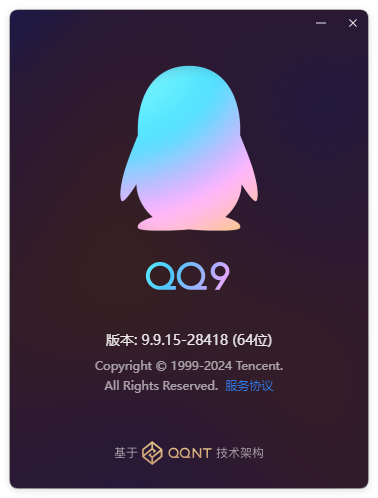
\includegraphics[width=\linewidth]{pic/NTQQ.png}
        \end{center}
    \end{minipage}

    \footnotetext[21]{\href{https://v2ex.com/t/955040}{2023年有哪些原生级性能的跨平台框架?} - V2EX}
    \footnotetext{\href{https://github.com/ShirasawaSama/CefDetectorX}{CEF检测器}}
\end{frame}

\begin{frame}[t]{就不告诉你:编程语言的小秘密}
    \fparbox[Br,boxrule=5pt,boxsep=10pt]{\textrm{第一个程序员\href{https://en.wikipedia.org/wiki/Ada_Lovelace}{爱达·勒芙蕾丝夫人}写了一个利用分析机计算伯努利数的程序}}\newline
    
    \alert{汇编(Assembly)}:隐藏了电路细节、硬件规范
    \begin{minipage}{0.7\linewidth}
        写出来往往“丑”但是快 \\
        现代汇编器如nasm远远强于原始汇编 \\[1em]
        每个年代举三个高级语言\footnotemark
        \begin{itemize}
            \item 1950s: FORTRAN(1955), LISP(1958), ALGOL58(1958)
            \item 1970s: PASCAL(1970), C(1972), SQL(1978)
            \item 1980s: Ada(1980), C++(1980), Perl(1989)
            \item 1990s: Python(1991), Java(1995), JavaScript(1995)
            \item 2000s+: C\#(2001), Go(2009), Rust(2015)
        \end{itemize}
    \end{minipage}
    \begin{minipage}{0.28\linewidth}
        \centering
        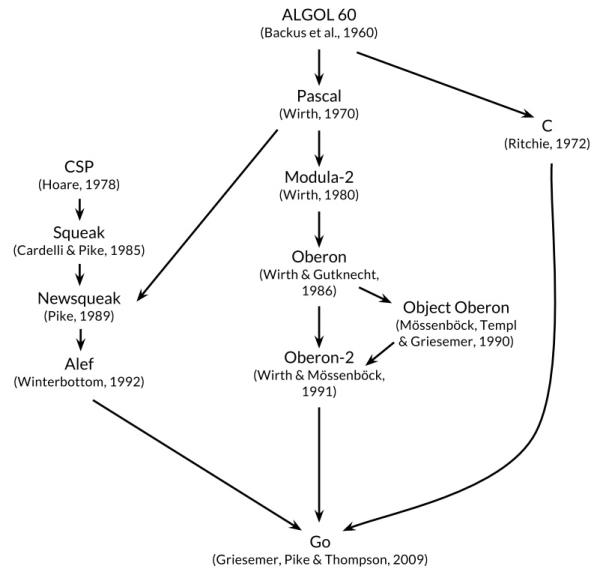
\includegraphics[width=\linewidth]{pic/GoDerivation.png}
    \end{minipage}
    \footnotetext{\href{https://en.wikipedia.org/wiki/History_of_programming_languages}{程式语言历史} - Wikipedia}
\end{frame}

\begin{frame}{Python和C:你在西财的必修课}
    还记得这个实时跟你交互的框框吗?\\ 或许你已经没用他而转向PyCharm了
    \begin{figure}[htb]
        \centering
        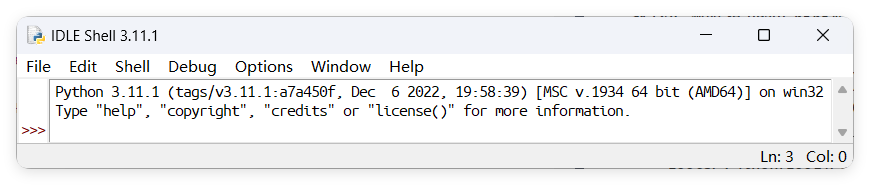
\includegraphics[width=0.5\textwidth]{pic/PythonREPL.png}
    \end{figure}
    他的正式命名叫做Python \href{https://en.wikipedia.org/wiki/Repl}{\alert{REPL/language shell}} \\[1em]

    解释型语言最早可以追溯到FORTRAN时期的 \href{https://en.wikipedia.org/wiki/Speedcoding}{Speedcoding} 上

    你知道为什么洛谷上的Python时间总是慢于C++吗?
    \begin{figure}[htb]
        \centering
        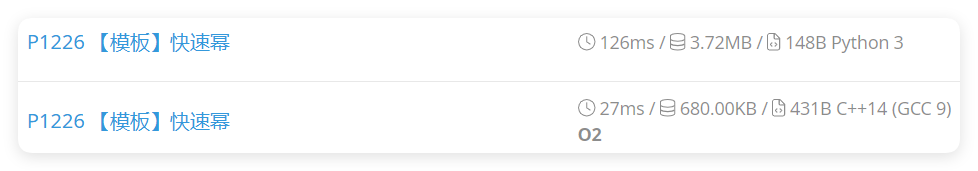
\includegraphics[width=0.5\textwidth]{pic/qpow.png}
    \end{figure}
\end{frame}

\begin{frame}{Python和C:你在西财的必修课 (cont'd)}
    \begin{minipage}{0.7\linewidth}
        为什么是C而不是其他语言?
        \begin{itemize}
            \item C本身就是为了UNIX而设计的\footnotemark
            \item C对硬件有极佳的操控性
            \item 出现时间早,有较为成熟的规范...
            \item 其实C语言也婆婆妈妈的
        \end{itemize}
    
        最受欢迎的现代语言:\href{https://stackoverflow.blog/2021/03/15/getting-started-with-rust/}{\alert{Rust}}\footnotemark
        \begin{itemize}
            \item 传闻最早是因为其发明者被困在电梯里面写的
            \item 考虑到了大部分程序员脑子不太灵光的问题
            \item 现有语言很难保证内存安全或仅有提案\footnotemark
            \item 借鉴了许多的语言,支持多种Paradigm...
        \end{itemize}
    \end{minipage}
    \begin{minipage}{0.28\linewidth}
        \centering
        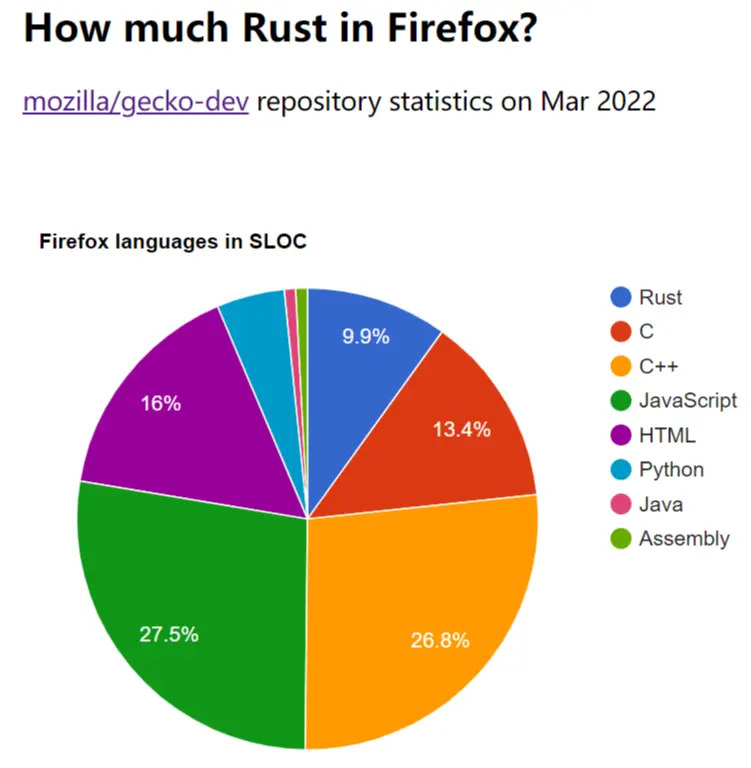
\includegraphics[width=\linewidth]{pic/MozillaRust.jpg}
    \end{minipage}

    \footnotetext[24]{\href{https://liuyandong.com/archives/10283}{第18届图灵奖、Unix与C语言发明者:肯·汤姆森与丹尼斯·里奇(DMR)}}
    \footnotetext[25]{\href{https://users.rust-lang.org/t/why-did-mozilla-adopt-rust/33009/4}{Why did Mozilla adopt Rust} - Rust Forum}
    \footnotetext{\href{https://safecpp.org/draft.html}{Safe C++草案}}
    \footnotetext{\href{https://www.whitehouse.gov/oncd/briefing-room/2024/02/26/press-release-technical-report/}{Future Software Should Be Memory Safe} - The White House}
\end{frame}

\begin{frame}[t]{开发环境也许并没有你想象的复杂}
    回忆一下你在Python课上学到的基本知识
    \begin{center}
        \begin{itemize}
            \item 编译器、解释器?为什么点一下按钮代码就跑起来了
            \item 为什么狗屎的IDLE没有及时检查语法,甚至是 \href{https://en.wikipedia.org/wiki/Monospaced_font}{\alert{Proportional font}}
            \item 一个合格的IDE需要?
        \end{itemize}
    \end{center}
    \begin{figure}
        \centering
        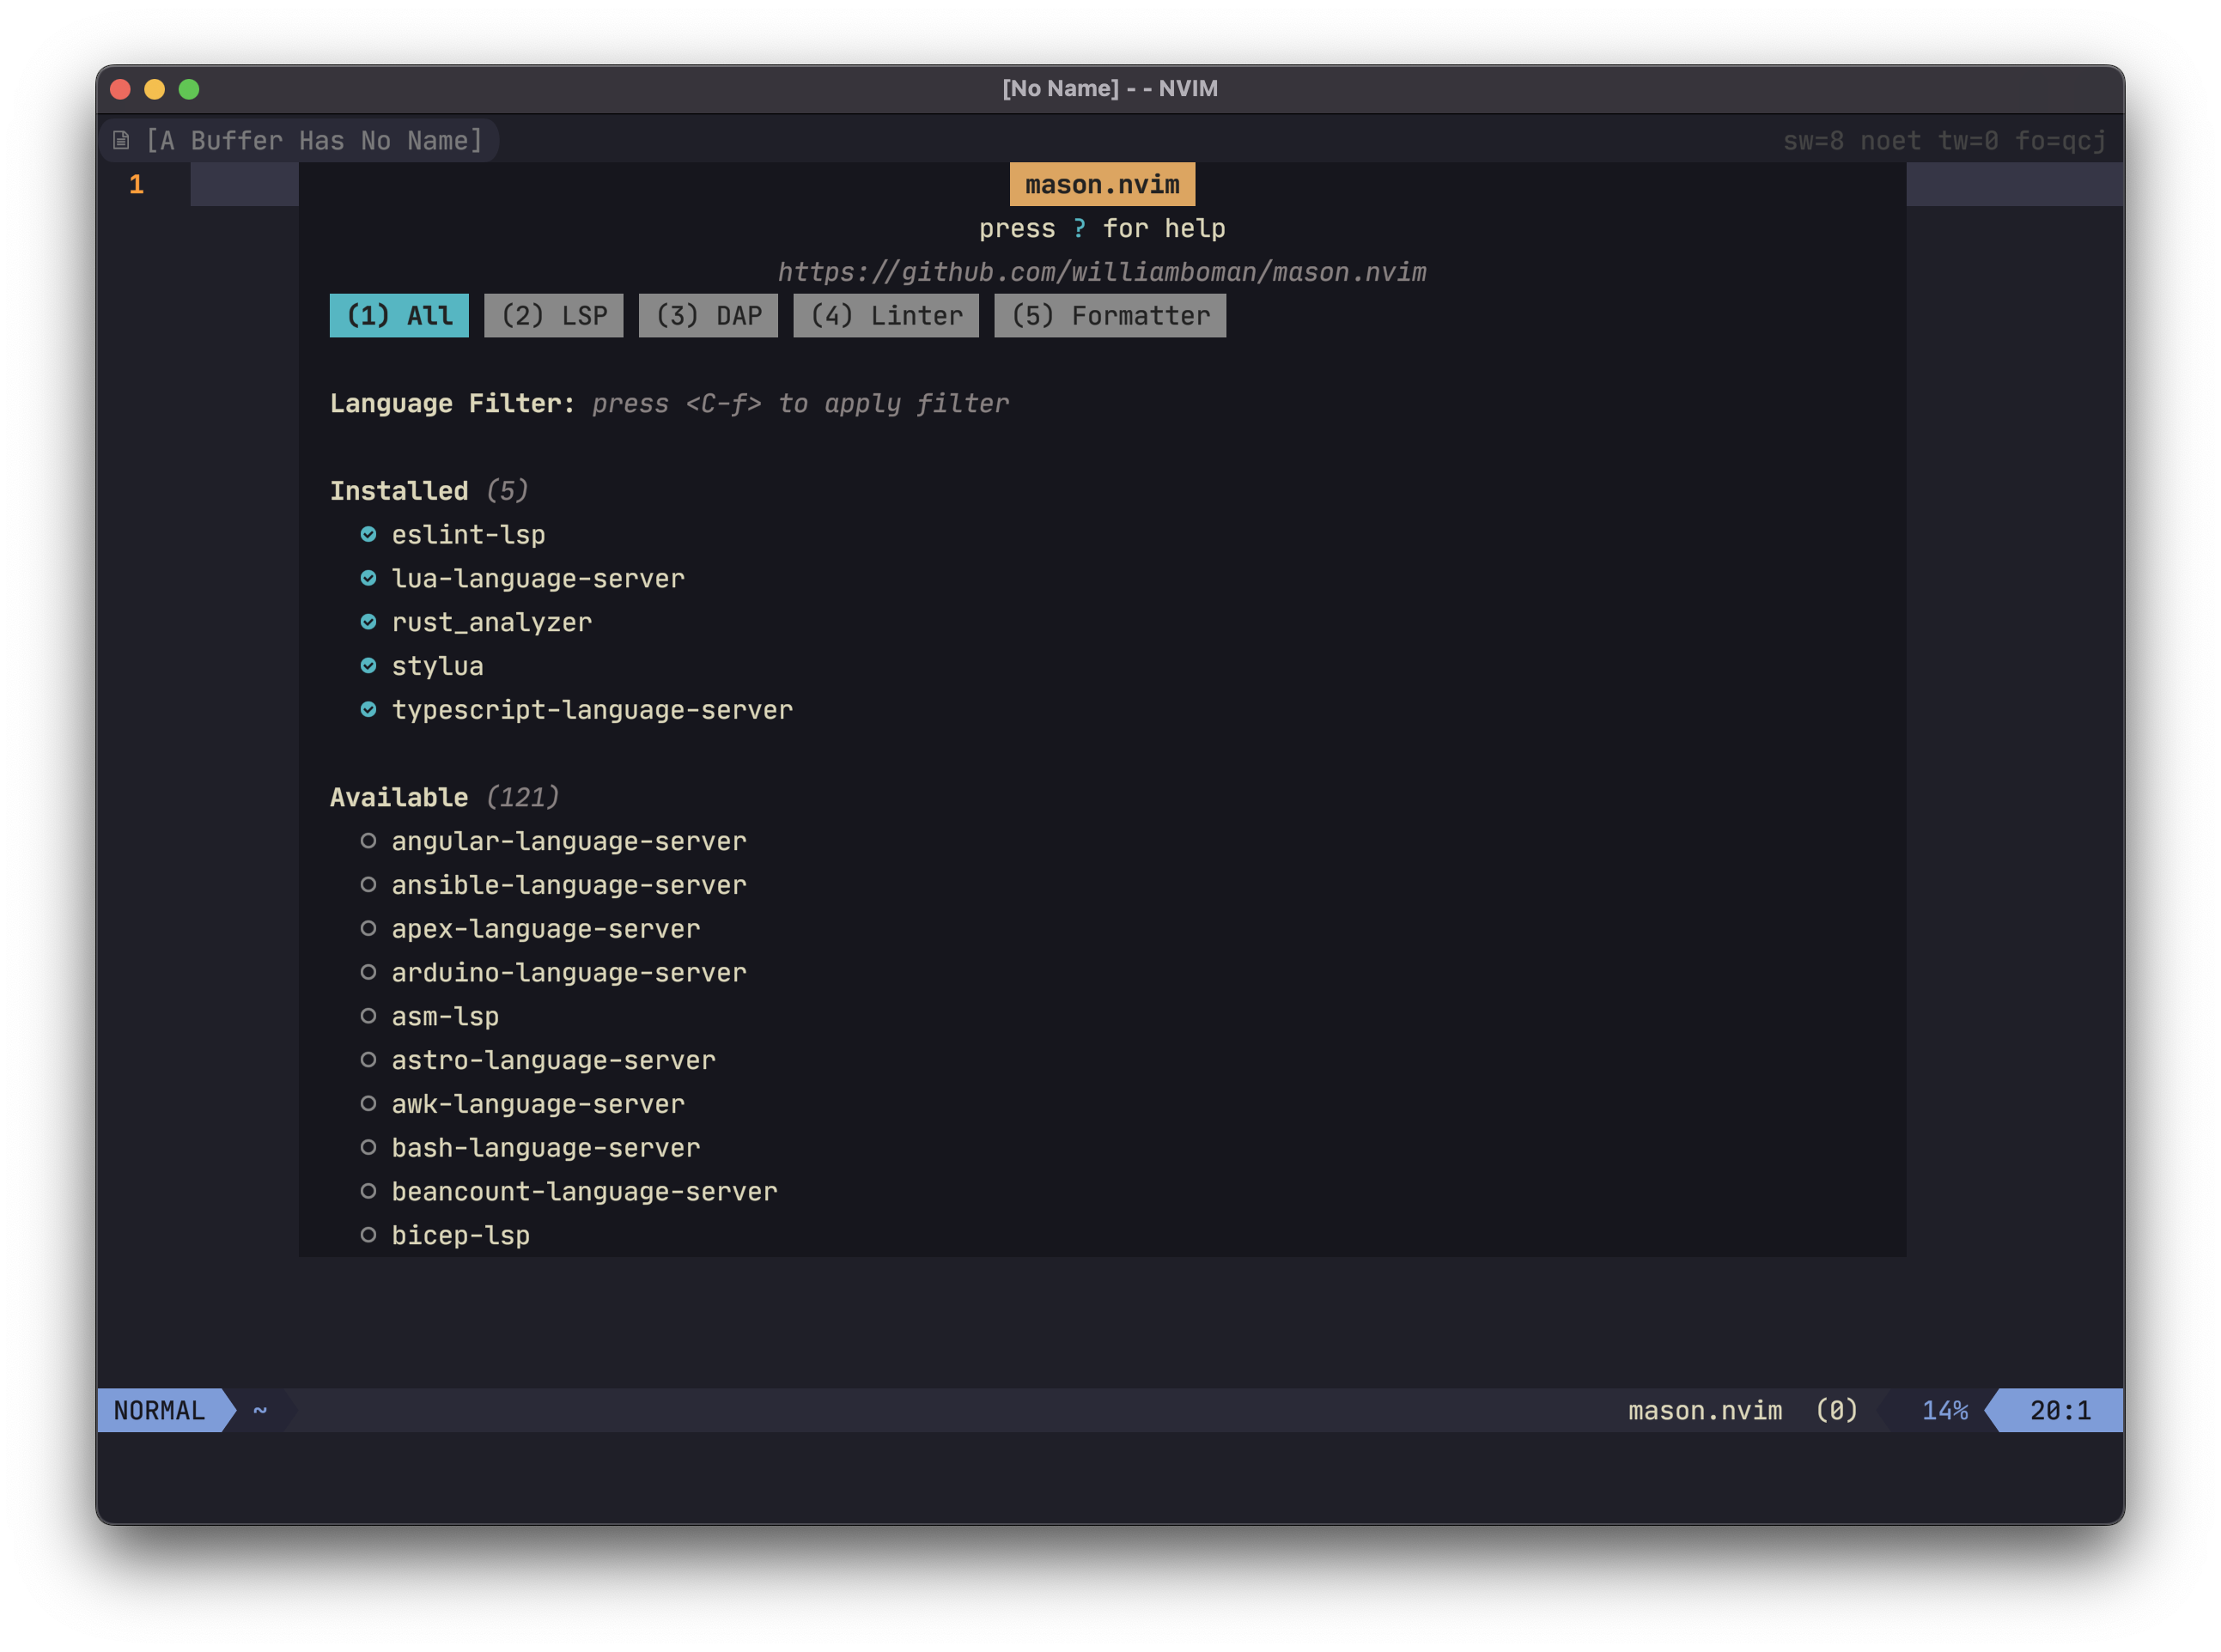
\includegraphics[width=0.5\textwidth]{pic/mason.png}
    \end{figure}
\end{frame}

\begin{frame}[t]{开发环境也许并没有你想象的复杂 (cont'd)}
    你的VSCode是怎么工作的?
    \begin{center}
        \begin{itemize}
            \item 你在无意识的享受着 \href{https://en.wikipedia.org/wiki/Language_Server_Protocol}{\alert{LSP}}(2016)带来的福利
            \item 也许AI工具真的会成为未来的发展趋势
            \item 许多编辑器开始朝着一些同样的方向发展 \href{https://unix.stackexchange.com/questions/57705/what-is-a-modeless-vs-a-modal-editor}{Modal editor}\ \href{https://www.cursor.com/}{Cursor}\ \href{https://www.vim.org/}{VIM}\ \href{https://helix-editor.com/}{Helix}
        \end{itemize}
    \end{center}
    \begin{figure}
        \centering
        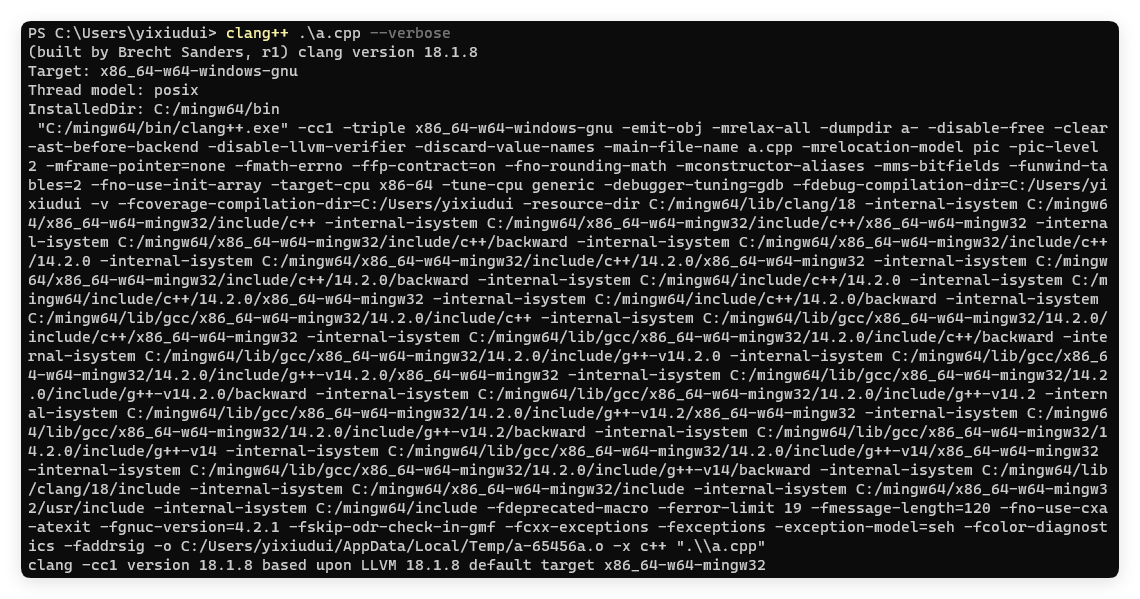
\includegraphics[width=0.6\textwidth]{pic/compile.png}
        \caption{这真的只是个简单的\texttt{Hello world}}
    \end{figure}
\end{frame}

\subsection{操作系统的启动过程}

\begin{frame}[t]{回顾组成原理}
    \fparbox[Br,boxrule=5pt,boxsep=10pt]{\textrm{CPU架构:IA32、IA64、AMD64、EM64T、RISC-V、MIPS、PowerPC...}}\newline
    
    我们以8086为例
    \begin{center}
        \begin{itemize}
            \item CPU上有很多寄存器(Register),每个寄存器由一些触发器(Flip-flop)组成
            \item 参数传递由操作系统做出规范,最重要的是 \alert{CS} 和 \alert{IP}
            \item CS是段地址,IP是段内偏移量,CS+IP就是指令的位置
            \item CPU开机时会有一个\alert{初始状态}\footnote{\href{https://www.intel.com/content/www/us/en/developer/articles/technical/intel-sdm.html}{IA64\&IA32 Architectures Software Developer’s Manual, Volume 3A/3B}},第一个访问的存储器是固件(Firmware)
            \item 针对不同架构我们必须用汇编启动\footnote{\href{https://github.com/torvalds/linux/blob/master/arch/x86/boot/header.S}{header.S} - Github torvalds/linux}...
        \end{itemize}
    \end{center}
\end{frame}

\begin{frame}{先来做些规范吧?}
    连启动方式也有差异?!
    \begin{center}
        \begin{itemize}
            \item 上面我们说的只针对MBR+Legacy(BIOS)启动\ 早已脱离时代潮流
            \item GPT+ \sout{\alert{MS-ish}}\footnotemark\ \href{https://uefi.org/specifications}{UEFI}\footnotemark 才是主流的启动方案
            \item \href{https://zhuanlan.zhihu.com/p/658162172}{coreboot} 也许小众,但谁更快更强不好说?
        \end{itemize}
    \end{center}
    \begin{figure}
        \centering
        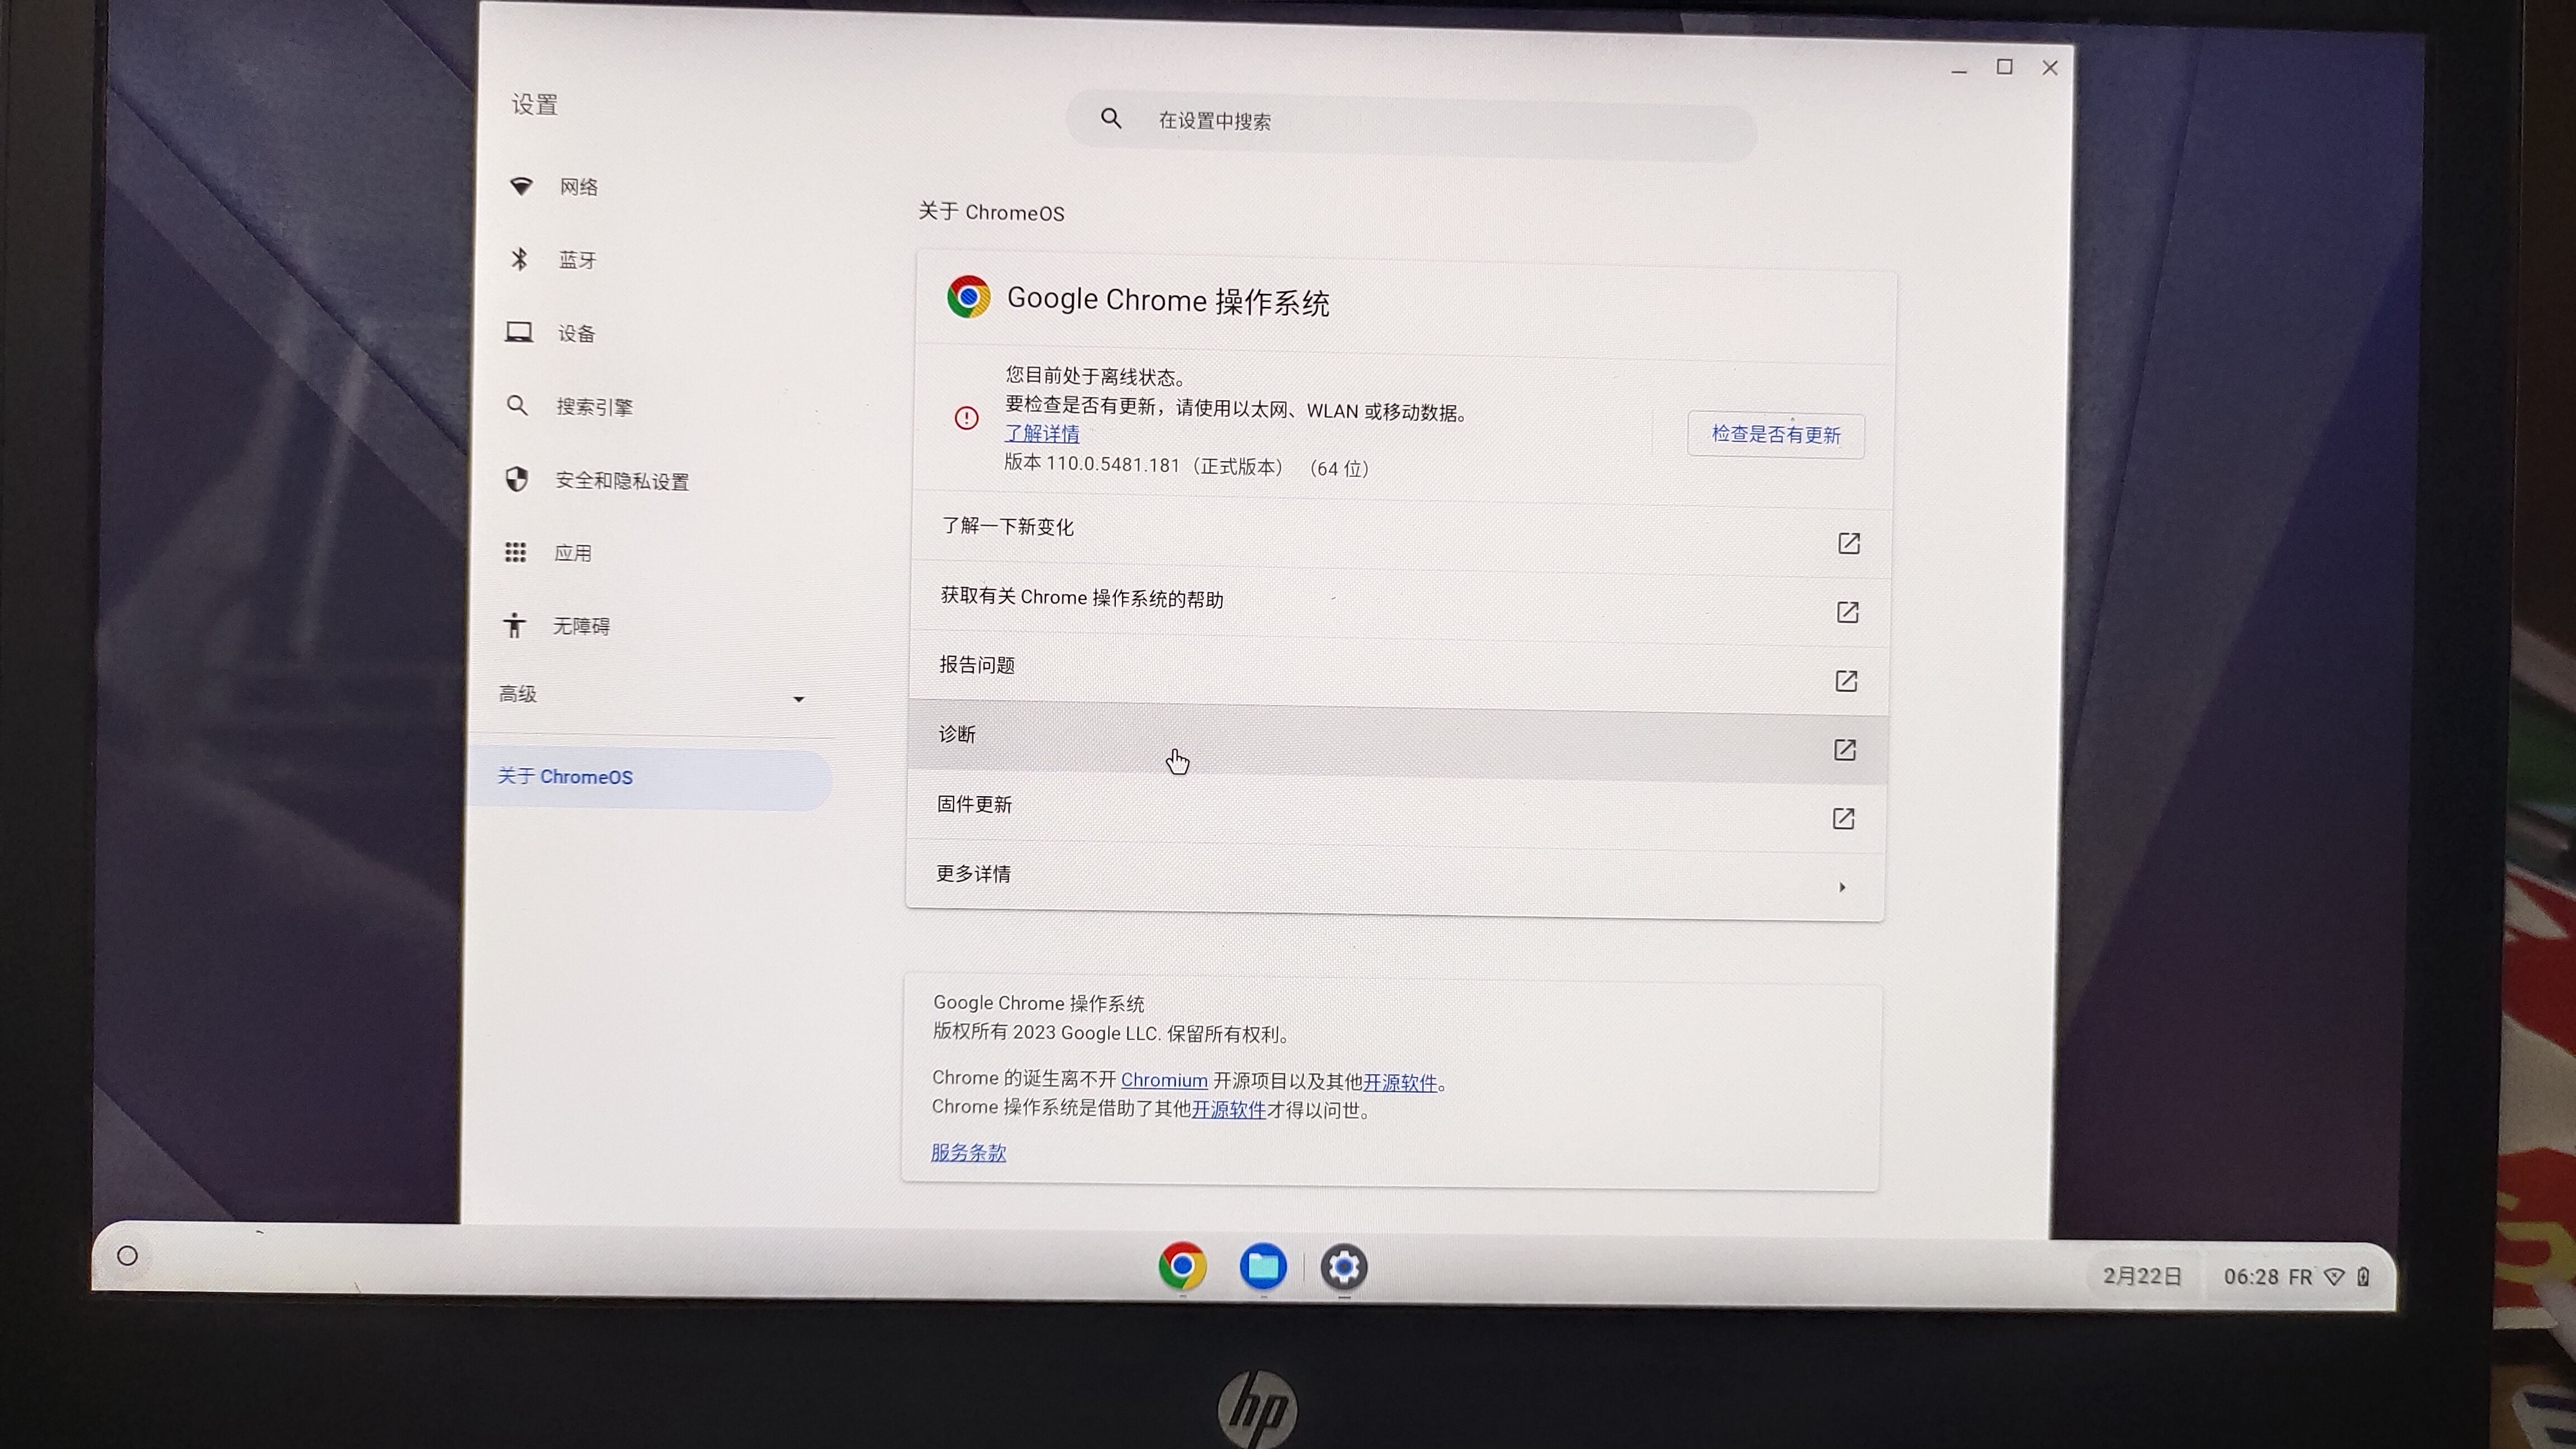
\includegraphics[width=0.47\textwidth]{pic/Chromebook.jpg}
    \end{figure}
    \footnotetext[29]{\href{https://www.zhihu.com/question/610490718/answer/3346377920}{为什么厂商都想推UEFI而不想让用户用BIOS呢?} - 韩朴宇的回答 - 知乎}
    \footnotetext[29]{\href{https://learn.microsoft.com/zh-cn/windows-hardware/design/device-experiences/oem-secure-boot}{安全启动} - Microsoft Learn}
    \footnotetext{\href{https://www.bilibili.com/video/BV1fm4y1q7Ns/}{GNU/Linux系统是如何启动的?} - 小刘不是程序员}
    \footnotetext{\href{https://wiki.archlinux.org/title/EFI_boot_stub}{EFISTUB} - ArchWiki}
\end{frame}

\begin{frame}{先来做些规范吧?(cont'd)}
    MBR的缺陷\footnote{\href{https://learn.microsoft.com/zh-cn/troubleshoot/windows-server/backup-and-storage/guid-partitioning-table-disk-faq}{有关 GUID 分区表磁盘体系结构的常见问题} - Microsoft Learn}
    \begin{center}
        \begin{itemize}
            \item 挂载(mount)和盘符的不确定性
            \item 单个分区大小不能超过2TB
            \item 主分区最多4个,或者只能有3个主分区+1个扩展分区
            \item 固件大小越来越充裕...
            \item 了解Grub2和Windows BootManager
        \end{itemize}
    \end{center}

    常用的文件系统
    \begin{center}
        \begin{itemize}
            \item NTFS(Windows)、ReFS(Windows server)
            \item FAT16、FAT32、exFAT(统称为vFAT)
            \item ext2、ext3、ext4(大部分Linux默认,部分安卓)
            \item APFS(MacOS)
            \item New generation:zfs, btrfs, xfs...
        \end{itemize}
    \end{center}
\end{frame}

\subsection{电源管理}

\begin{frame}{其他的模块可能无感但这个真不行:ACPI}
    相比于APM把电源控制权全部交给BIOS,ACPI能够更加精细的控制系统能耗 \\[1em]

    ACPI定义了一些“状态”\footnote{\href{https://en.wikipedia.org/wiki/ACPI}{ACPI} - Wikipedia}:全局状态、电源状态、处理器性能状态... \\
    我们比较关心的是全局状态(Global state)
    \begin{minipage}{0.6\linewidth}
        \begin{center}
            \begin{itemize}
                \item G0:正常工作状态
                \item G1:睡眠状态
                    \begin{itemize}
                        \item \alert{S0:Modern standby}
                        \item S1:Power on Suspend
                        \item S2:deprecated
                        \item S3:Suspend to RAM(Sleep/Standby)
                        \item S4:Suspend to Disk(Hibernate)
                    \end{itemize}
                \item G2:Soft off
                \item G3:Mechanical off
            \end{itemize}
        \end{center}
    \end{minipage}
    \begin{minipage}{0.3\linewidth}
        \centering
        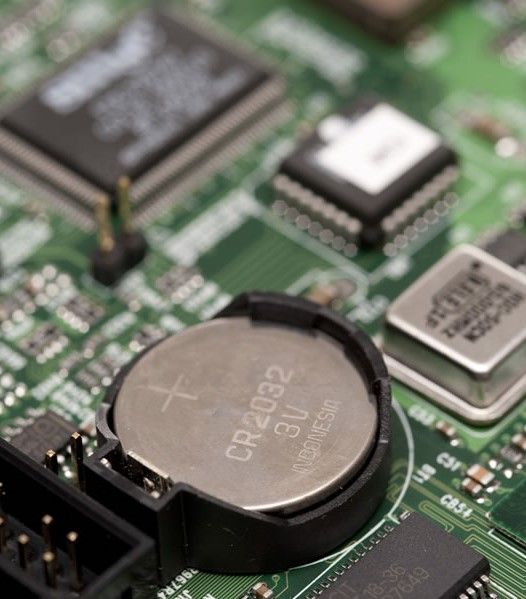
\includegraphics[width=\linewidth]{pic/lithium_bios_battery.jpg}
    \end{minipage}

    \footnotetext[32]{\href{https://edc.intel.com/content/www/us/en/design/ipla/software-development-platforms/client/platforms/alder-lake-desktop/12th-generation-intel-core-processors-datasheet-volume-1-of-2/advanced-configuration-and-power-interface-acpi-states-supported/}{Intel 12th Gen ACPI States Supported} - Intel}
    \footnotetext[32]{\href{https://learn.microsoft.com/zh-cn/windows-hardware/drivers/kernel/system-sleeping-states}{系统睡眠状态} - Microsoft Learn}
\end{frame}

\begin{frame}{其他的模块可能无感但这个真不行:ACPI (cont'd)}
    \begin{minipage}{0.48\linewidth}
        你遇到过这种情况吗?
        \begin{itemize}
            \item 充着电玩电脑,用完过后随手一拔电放包里,第二天发现已经没电了
            \item 上节课写代码,写完过后电脑合盖放包里,下节课一取出来后盖滚烫
            \item 你正在使用Windows\footnotemark
            \item 你的电脑关机很快启动很快耗电也很快\footnotemark
        \end{itemize}
    \end{minipage}
    \begin{minipage}{0.25\linewidth}
        \flushright
        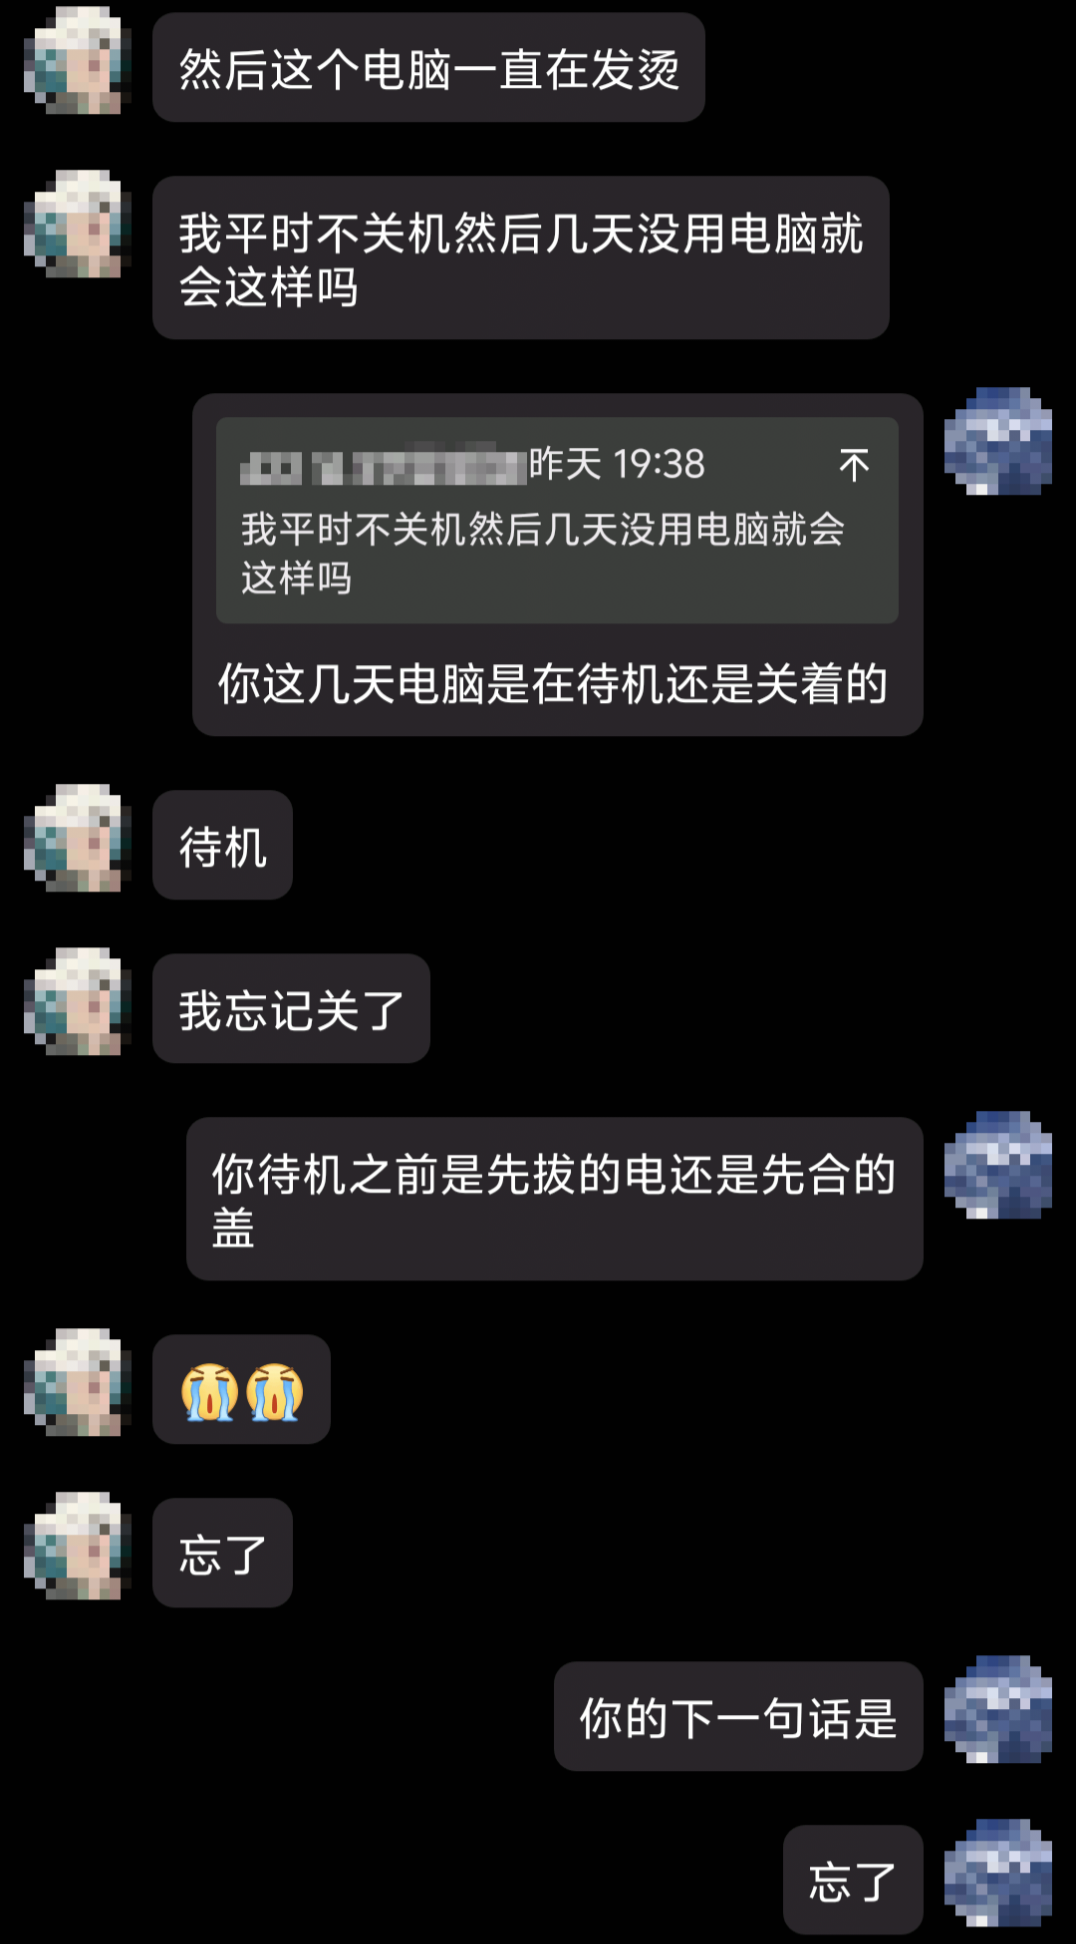
\includegraphics[width=\linewidth]{pic/123.png}
    \end{minipage}
    \begin{minipage}{0.25\linewidth}
        \flushright
        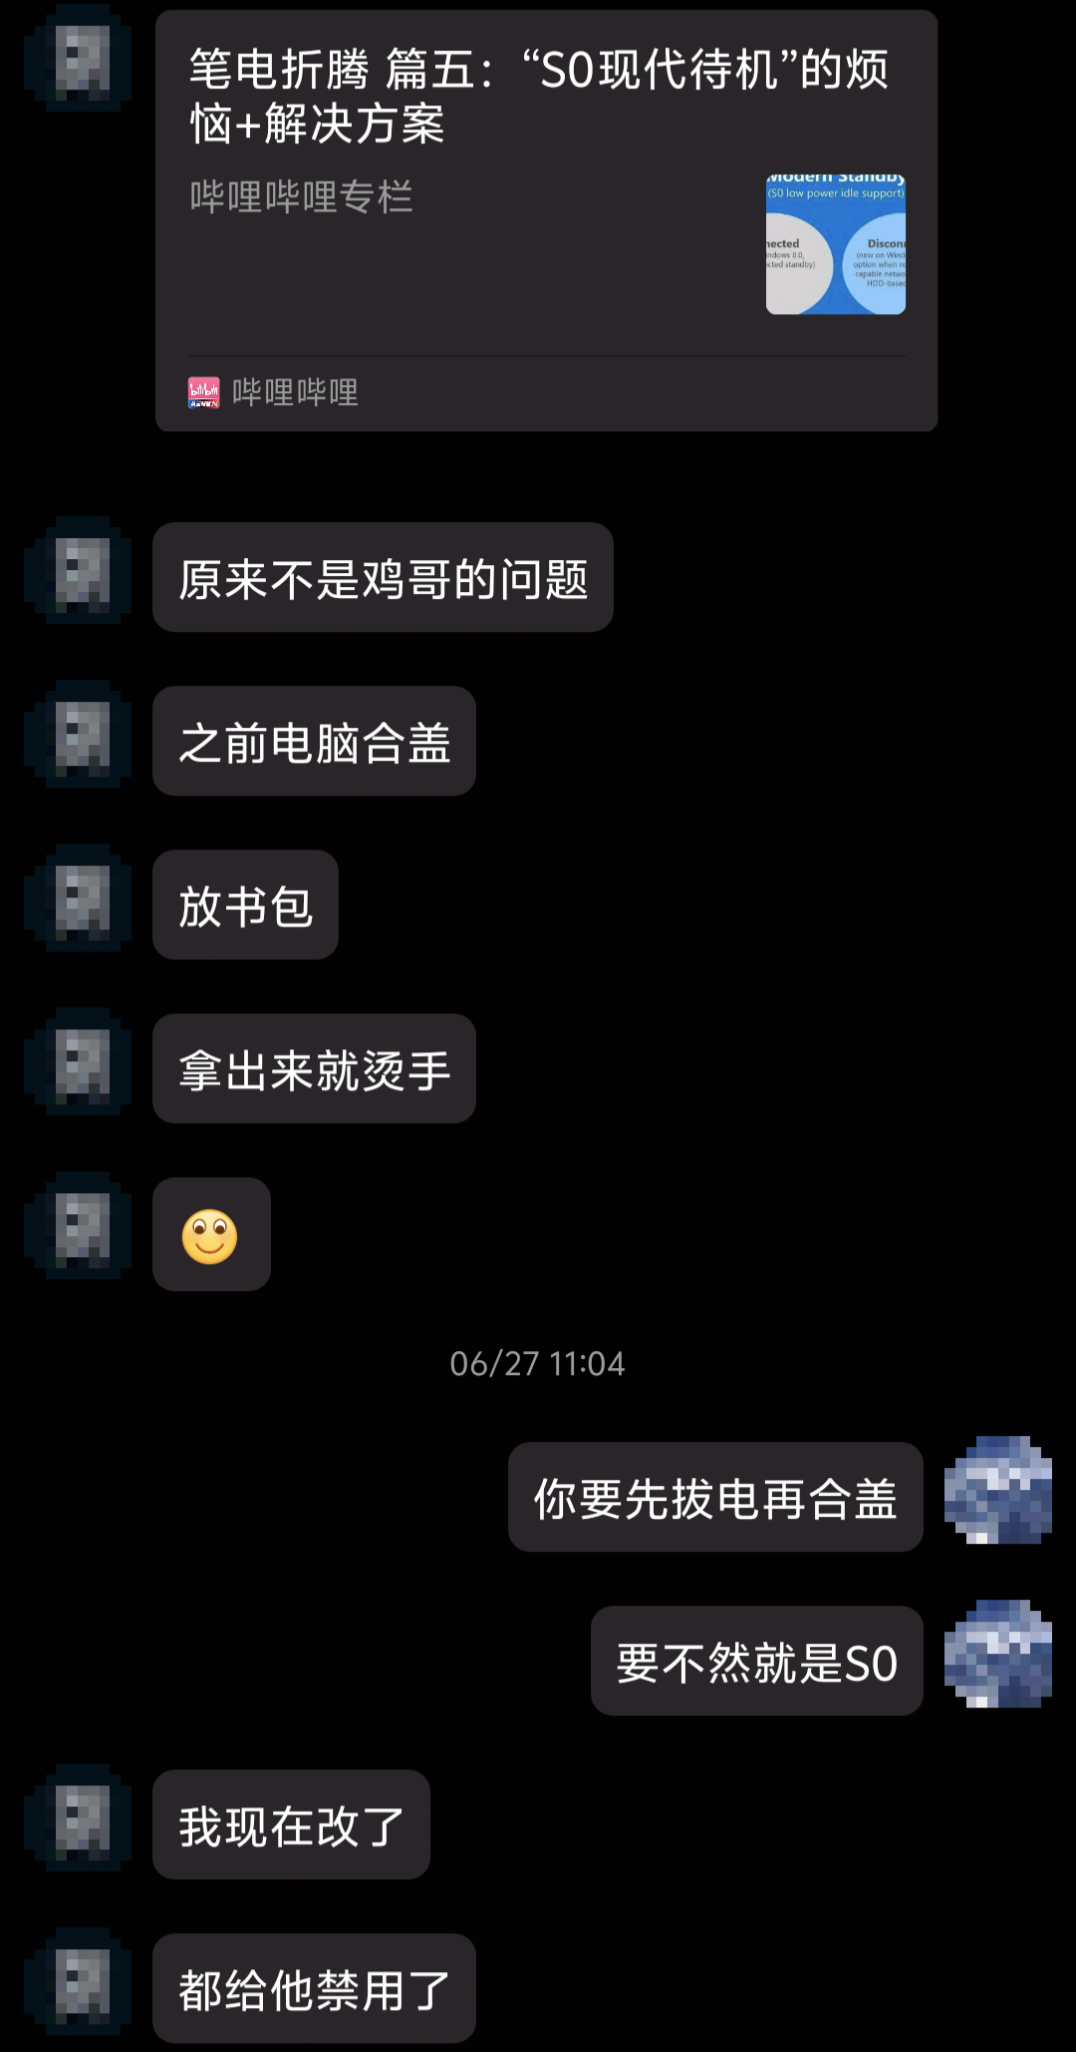
\includegraphics[width=\linewidth]{pic/456.png}
    \end{minipage}

    \footnotetext[33]{\href{https://www.bilibili.com/video/BV1Pv4y1d7Ms}{微软这是在逼我买MacBook--Windows新式待机} - LinusTechTips}
    \footnotetext{\href{https://web.archive.org/web/20240614042327/https://tedstechshack.com/2017/07/03/warning-multi-booting-uefi-system-windows-10-fast-startup-doubt-reboot/}{注意双系统情况下的Windows快速启动...} - Ted's Tech Shack}
\end{frame}

\subsection{Ventoy}

\begin{frame}{Ventoy:好用的小工具}
    相信你们都用过光碟,放过电影听过歌
    \begin{center}
        \begin{itemize}
            \item 事实上,早期的很多软件安装都是通过光盘来完成的
            \item 光盘里面的东西就是一个ISO9660文件(包含了文件系统信息)
        \end{itemize}
    \end{center}

    你并不需要把U盘看得很特殊,U盘和硬盘都属于\alert{持久化介质}
    \begin{center}
        \begin{itemize}
            \item 光盘拔掉即消失
            \item 即使是WinPE,也是加载到内存中的系统
            \item Ventoy就是把镜像当成光盘来实现的\footnote{\href{https://www.ventoy.net/cn/compatible.html}{Compatible} - Ventoy}
        \end{itemize}
    \end{center}
    \begin{figure}
        \centering
        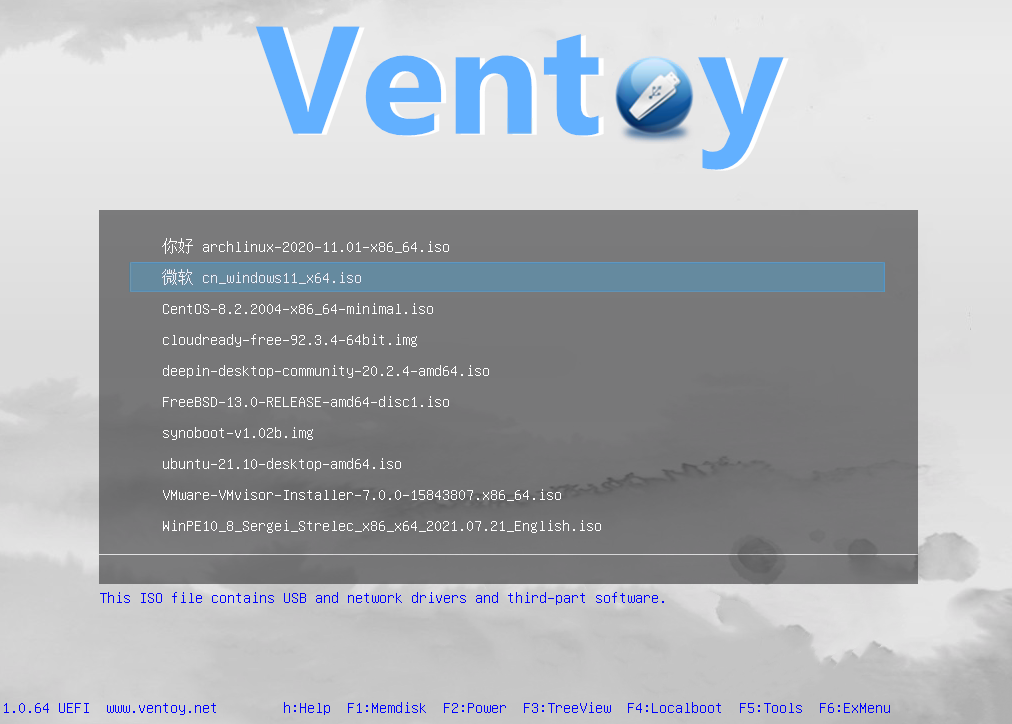
\includegraphics[width=0.29\linewidth]{pic/screen_uefi.png}
    \end{figure}
\end{frame}

\section{实机操作}

\begin{frame}{实验一}
    使用Ventoy中的FirPE安装Windows
\end{frame}

\begin{frame}{实验二}
    \begin{center}
        \begin{itemize}
            \item 完成双系统安装(Arch Linux with \texttt{archinstall})
            \item 了解挂载思想
            \item 了解lvm2
        \end{itemize}
    \end{center}
\end{frame}
\section{其他资料}

\begin{frame}{Olympiad in Informatics (OI)}
    \begin{minipage} {0.6\linewidth}
        \centering
        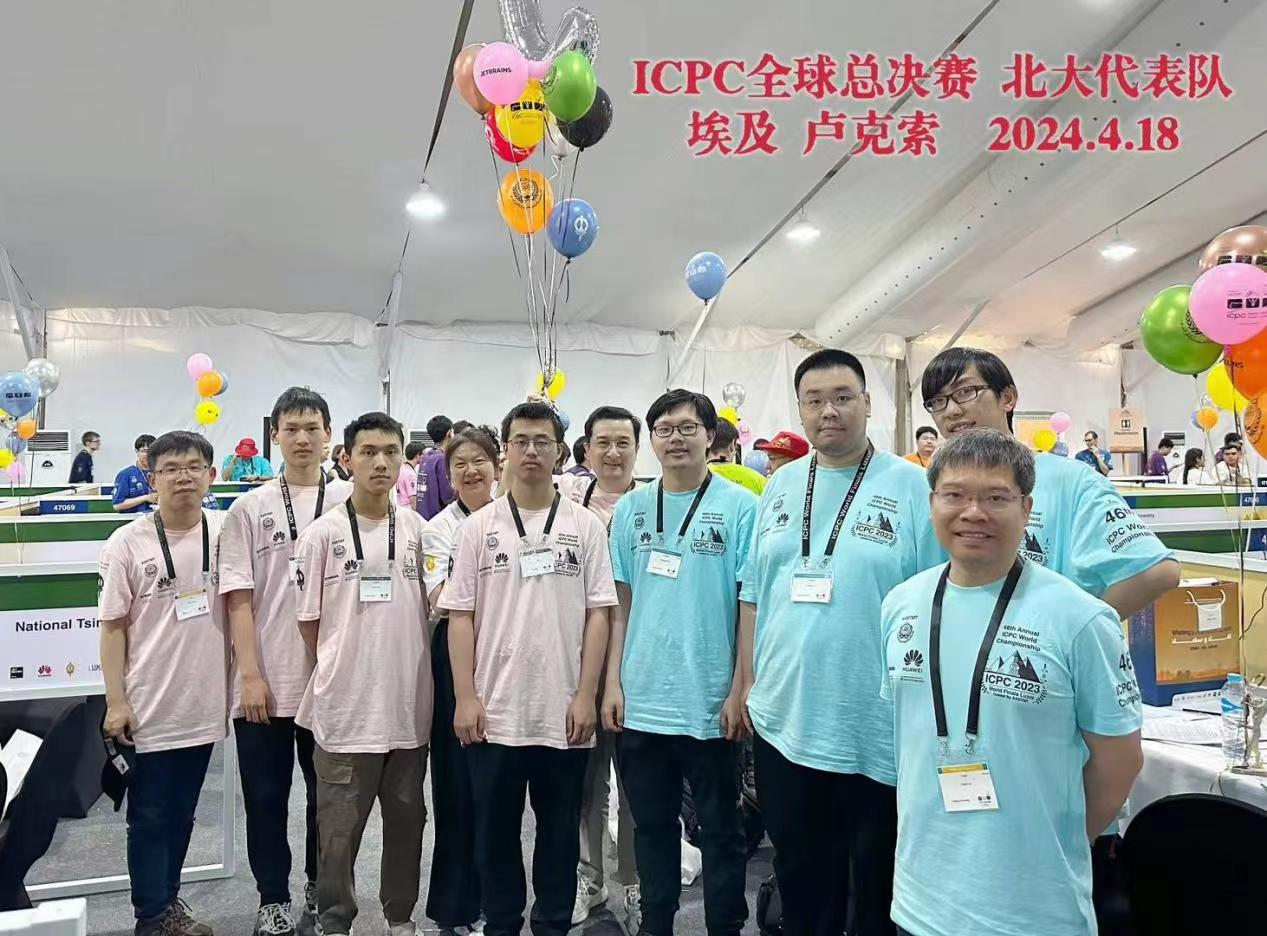
\includegraphics[width=0.8\linewidth]{pic/OI.jpg}
    \end{minipage}
    \begin{minipage}{0.38\linewidth}
        大学生能够参加的信息学赛事
        \begin{center}
            \begin{itemize}
                \item ICPC
                \item CCPC
                \item 蓝桥杯
                \item 天梯赛(团队赛)
                \item 百度之星
                \item CCF CSP、CCSP...
            \end{itemize}
        \end{center}
    
        网络赛网站
        \begin{center}
            \begin{itemize}
                \item \href{https://codeforces.com}{Codeforces}
                \item \href{https://atcoder.jp}{AtCoder}
                \item \href{https://ac.nowcoder.com/}{牛客}
                \item \href{https://luogu.com.cn/}{洛谷}
            \end{itemize}
        \end{center}
    \end{minipage}
\end{frame}

\begin{frame}{如何查找资料}
    \begin{minipage}{0.63\linewidth}
        前提:\href{https://integrity.mit.edu/}{\alert{学术诚信}}
        \begin{center}
            \begin{itemize}
                \item RTFM,STFW,RTFSC
                \item \href{https://wikipedia.org}{Wikipedia}
                \item 多阅读来源可信的信息:\\ 学术会议、久经考验的论文或Tutorial \\ 选择Stackoverflow而不是CSDN \\ 选择Google或DuckduckGo而不是百度 \\ 使用英语检索关键词、多看官方论坛
                \item 使用“对的”自动化工具
                \item 保持你的热爱
                \item \sout{加入CAAC}
                \item 多问问师傅吧$\backslash\textrm{哭}$ \\ 本人主要学习领域:\\ OS、PL、Architecture
            \end{itemize}
        \end{center}
    \end{minipage}
    \begin{minipage}{0.35\linewidth}
        \centering
        
\includegraphics[width=\linewidth]{pic/userFriendly.png}
    \end{minipage}
\end{frame}

\begin{frame}{义修队日常工作}
    \begin{itemize}
        \item 值班
        \item 外勤
        \item 义诊
        \item 记得看群文件教程!!!!!!!!!!
        \item 约饭
    \end{itemize}
\end{frame}

\section{更多内容}

\begin{frame}{更多知识...}
    \begin{itemize}
        \item 字体设计,字体渲染
        \item WebAssembly
        \item Tiling WM, stacking WM
        \item ELF,EXE,COM...
        \item 自动化工具 makefile,CMake
        \item SFU,WSA(deprecated),WSL,KVM,Hyper-V...
        \item Modern programming language
        \item 网络开发的前端后端
        \item 函数式编程(Functional programming)
        \item 分布式(Distributed),高性能计算(HPC)
        \item 形式化的数学模型,回归到Turing machine和State machine
        \item 对国产化的思考\ \href{https://github.com/microsoft/vscode/issues/191229}{CEC-IDE}
    \end{itemize}
\end{frame}

\begin{frame}{推荐阅读}
    手册
    \begin{itemize}
        \item 为什么UNIX family如此庞大?\ \href{https://pubs.opengroup.org/onlinepubs/9799919799/index.html}{POSIX Conventions(现在叫SUS)}
        \item 函数参数到底怎么传递的?\ \href{https://gitlab.com/x86-psABIs/x86-64-ABI}{x86-64 SystemV ABI}
        \item 更多关于Linux的组成、设计(需要一定基础)\ \href{https://www.linuxfromscratch.org/}{Linux From Scratch}
    \end{itemize}

    论文
    \begin{itemize}
        \item \href{https://people.freebsd.org/~lstewart/articles/cpumemory.pdf}{What Every Programmer Should Know About Memory}
        \item \href{http://ithare.com/infographics-operation-costs-in-cpu-clock-cycles/}{Operation Costs in CPU Clock Cycles}
        \item \href{https://courses.cs.washington.edu/courses/cse550/20au/papers/CSE550.Atlas.pdf}{The Manchester Mark I and Atlas: A Historical Perspective}
    \end{itemize}

    推荐课程
    \begin{itemize}
        \item \href{https://nju-projectn.github.io/ics-pa-gitbook/}{南京大学ICS PA}
        \item \href{https://jyywiki.cn/OS/2024/}{南京大学操作系统}
        \item \href{https://web.stanford.edu/class/cs143/}{Stanford CS143 Compilers}
        \item \href{https://missing.csail.mit.edu/}{MIT The Missing Semester of Your CS Education}
    \end{itemize}

    OS和编译原理属于\alert{高阶课程},但并不意味着不能一步一步地深入了解他们,使用他们;上面的大部分内容并不是操作系统课程或者编译原理课程的主要内容,但往往是更加有趣,更为实用的
\end{frame}

% \begin{frame}[allowframebreaks]
%     \bibliography{ref}
%     \bibliographystyle{alpha}
%     % 如果参考文献太多的话,可以像下面这样调整字体:
%     % \tiny\bibliographystyle{alpha}
% \end{frame}

\begin{frame}
    \begin{center}
        {\Huge\calligra Fin.}
    \end{center}
\end{frame}

\end{document}